% % Preamble BEGINN %%%%%%%%%%%%%%%%%%%%%%%%%%%%%%%%%%%%%%%%%%%%%%%%%%%%%%%%%

%%% Preamble (Dokumentenklasse)
% ------------------------------------------------------------------------
% LaTeX - Preambel ******************************************************
% ------------------------------------------------------------------------
% Dokumentklasse (Koma Script)
% ------------------------------------------------------------------------
% basiernd auf www.matthiaspospiech.de/latex/vorlagen Diplomarbeit kompakt
% ========================================================================
\documentclass[%
   %draft,            % Entwurfsstadium
   final,             % fertiges Dokument
   12pt,              % Schriftgroesse der Grundschrift
   bigheadings,       % gro�e �berschriften
   ngerman,           % wird an andere Pakete weitergereicht
   a4paper,           % Papierformat
   BCOR5mm,          % Bindekorrektur: Zus�tzlicher Rand auf der Innenseite
   DIV14,            % Seitengr��e (siehe Koma Skript Dokumentation !)
   1.1headlines,     % Zeilenanzahl der Kopfzeilen
   pagesize,         % Schreibt die Papiergroesse in die Datei.
   oneside,          % Einseitiges Layout
%   twoside,          % Zweiseitiges Layout
   openright,        % Kapitel beginnen immer auf der rechten Seite
   titlepage,        % Titel als einzelne Seite ('titlepage' Umgebung)  
   headsepline,      % Linie unter Kolumnentitel ()
%   plainheadsepline, % Linie unter Kolumnentitel () plain Seitenstil
   nochapterprefix,  % keine Ausgabe von 'Kapitel:'
   bibtotoc,         % Bibliographie ins TOC
%	bibtotocnumbered, % Bibliographie ins TOC mit Kapitelnummer
   tocindent,        % eingereuckte Gliederung
   listsindent,      % eingereuckte LOT, LOF
   pointlessnumbers, % �berschriftnummerierung ohne Punkt, siehe DUDEN !
   cleardoubleempty, % Leere linke Seite bei Zweiseitenlayout vor Kapitel
   fleqn,            % Formeln werden linksbuendig angezeigt
%   parindent,        % Absatz mit Einzug (Standard)
   halfparskip,      % Absatz halbe Zeile Abstand
%   parskip,          % Absatz ganze Zeile Abstand
]{scrbook}%     Klassen: scrartcl, scrreprt, scrbook


%%% Alle Namen usw. im Titel und im hyperref-Paket
% ------------------------------------------------------------------------
% LaTeX - Preambel ******************************************************
% ------------------------------------------------------------------------
% pre-work
% ========================================================================
% % ToDo kennzeichnen
\newcommand{\workTodo}[1]{\textcolor{red}{todo: #1}}

% % F�r Datum und Zeit in Fusszeile
% % !!!Inhalt bei Fertigstellung der Arbeit l�schen
\newcommand{\workMarkDateTime}{\today{}  }

% % Alle Namen werden im Titel und im hyperref-Paket eingetragen
% % !!! Ueberall f�r <Wert> das Entsprechende eintragen

 % <Typ> Studienarbeit, Dipolmarbeit, Studienarbeit oder Bachlor-Abschlussarbeit
\newcommand{\workTyp}{Team Project\xspace}

 % <Titel> der Arbeit
\newcommand{\workTitel}{Quadrocopter}

 % <Studiengang> z.B. Kommunikationstechnik
\newcommand{\workStudiengang}{ASM-SB \xspace}

% <Semester> mit Jahr z.B. Sommersemester 2008  
\newcommand{\workSemester}{ASM2\xspace}

% <Name> des Studenten
\newcommand{\workNameStudentOne}{Oliver Breuning\xspace}
\newcommand{\workNameStudentTwo}{Martin Brodbeck\xspace}
\newcommand{\workNameStudentThree}{J\"urgen Schmidt\xspace}
\newcommand{\workNameStudentFour}{Phillip Woditsch\xspace}

% <Pruefer> Name des pr�fenden (betreuenden) Professor an der Hochschule
\newcommand{\workPruefer}{Prof. Dr. J\"org Friedrich\xspace} 


% %%% Nur bei Abschluss-Arbeiten

% <Datum> der Abgabe der Arbeit (Eidesstatliche Erkl�rung)
\newcommand{\workDatum}{\today\xspace}

% <Zweitpr�fer>
\newcommand{\workZweitPruefer}{\workTodo{<Zweitpr�fer>}\xspace}

% <Zeitraum>
\newcommand{\workZeitraum}{Summersemester 2015\xspace}


% %%% Nur bei Industrie-Arbeiten:

% <Firma>
\newcommand{\workFirma}{\workTodo{<Firma>}\xspace}

% <Betreuer in der Firma>
\newcommand{\workBetreuer}{\workTodo{<Betreuer in der Firma>}\xspace}

% Firmenlogo Name hier anpassen, Gr��e (wenn m�glich) nicht �ndern
%\newcommand{\workFirmenLogo}{
\includegraphics[width=5cm]{fig/aa-titel/Bosch_4C_S}} 


%%% Preamble (Pakete)
% ------------------------------------------------------------------------
% LaTeX - Preambel ******************************************************
% ------------------------------------------------------------------------
% Packages
% ------------------------------------------------------------------------
% basiernd auf www.matthiaspospiech.de/latex/vorlagen Diplomarbeit kompakt
% ========================================================================

% Inhalt:
% 1. Einige Pakete muessen unbedingt vor allen anderen geladen werden
% 2. Fonts Fonts Fonts
% 3. Math Packages
% 4. Symbole
% 5. text related packages
% 6. Pakete zum Zitieren
% 7. PDF related packages
% 8. Tables (Tabular)
% 9. figures and placement
% 10. verbatim packages
% 11. science packages
% 12. layout packages

% ~~~~~~~~~~~~~~~~~~~~~~~~~~~~~~~~~~~~~~~~~~~~~~~~~~~~~~~~~~~~~~~~~~~~~~~~
% Encoding der Dateien (sonst funktionieren Umlaute nicht)
% Empfohlen latin1, da einige Pakete mit utf8 Zeichen nicht
% funktionieren, z.B: listings, soul.

\usepackage[latin1]{inputenx} % ISO-8859-1
%\usepackage[ansinew]{inputenx} % Windows-Standard (CP1252) (baut auf ISO 8859-1 und ISO 8859-15 auf)
%\usepackage[utf8]{inputenc}

% ~~~~~~~~~~~~~~~~~~~~~~~~~~~~~~~~~~~~~~~~~~~~~~~~~~~~~~~~~~~~~~~~~~~~~~~~
% 1. Einige Pakete muessen unbedingt vor allen anderen geladen werden
% ~~~~~~~~~~~~~~~~~~~~~~~~~~~~~~~~~~~~~~~~~~~~~~~~~~~~~~~~~~~~~~~~~~~~~~~~
%
\usepackage{xspace} % Define commands that don't eat spaces.
\usepackage{ifpdf} % Fuer Pakete/Paketoptionen, die nur fuer pdf benoetigt werden \ifpdf \else \fi
\usepackage{calc} % Calculation with LaTeX
\usepackage[english]{babel} % Languagesetting
\usepackage[table]{xcolor} % Farben
\usepackage[]{graphicx} % Bilder
%\usepackage{epstopdf} % If an eps image is detected, epstopdf is automatically called to convert it to pdf format.
\usepackage[]{amsmath} % Amsmath - Mathematik Basispaket
\usepackage{ragged2e} % Besserer Flatternsatz (Linksbuendig, statt Blocksatz)

% ~~~~~~~~~~~~~~~~~~~~~~~~~~~~~~~~~~~~~~~~~~~~~~~~~~~~~~~~~~~~~~~~~~~~~~~~
% 2. Fonts Fonts Fonts
% ~~~~~~~~~~~~~~~~~~~~~~~~~~~~~~~~~~~~~~~~~~~~~~~~~~~~~~~~~~~~~~~~~~~~~~~~

\usepackage[T1]{fontenc} % T1 Schrift Encoding (notwendig f�r die meisten Type 1 Schriften)
\usepackage{textcomp}	 % Zusatzliche Symbole (Text Companion font extension)

% Alle Schriften die hier angegeben sind sehen im PDF richtig aus.
% Die LaTeX Standardschrift ist die Latin Modern (lmodern Paket).
% If Latin Modern is not available for your distribution you must install the
% package cm-super instead. Otherwise your fonts will look horrible in the PDF

% DO NOT LOAD ae-Package for the font !

%% - Latin Modern
\usepackage{lmodern}
%% -------------------
%
% % - Times, Helvetica, Courier (Word Standard...)
%\usepackage{mathptmx}
%\usepackage[scaled=.90]{helvet}
%\usepackage{courier}
% % -------------------
%%
%% - Palantino , Helvetica, Courier
%\usepackage{mathpazo}
%\usepackage[scaled=.95]{helvet}
%\usepackage{courier}
%% -------------------
%
%% - Bera Schriften
%\usepackage{bera}
%% -------------------
%
%% - Charter, Bera Sans
%\usepackage{charter}\linespread{1.05}
%\renewcommand{\sfdefault}{fvs}


% ~~~~~~~~~~~~~~~~~~~~~~~~~~~~~~~~~~~~~~~~~~~~~~~~~~~~~~~~~~~~~~~~~~~~~~~~
% 3. Math Packages
% ~~~~~~~~~~~~~~~~~~~~~~~~~~~~~~~~~~~~~~~~~~~~~~~~~~~~~~~~~~~~~~~~~~~~~~~~

\usepackage[fixamsmath,disallowspaces]{mathtools} % Erweitert amsmath und behebt einige Bugs
\usepackage{fixmath}
\usepackage[all,warning]{onlyamsmath} % Warnt bei Benutzung von Befehlen die mit amsmath inkompatibel sind.
\usepackage{icomma} % Erlaubt die Benutzung von Kommas im Mathematikmodus

% ~~~~~~~~~~~~~~~~~~~~~~~~~~~~~~~~~~~~~~~~~~~~~~~~~~~~~~~~~~~~~~~~~~~~~~~~
% 4. Symbole
% ~~~~~~~~~~~~~~~~~~~~~~~~~~~~~~~~~~~~~~~~~~~~~~~~~~~~~~~~~~~~~~~~~~~~~~~~
\usepackage{amssymb}
%\usepackage{wasysym}
%\usepackage{marvosym}
%\usepackage{pifont}

% ~~~~~~~~~~~~~~~~~~~~~~~~~~~~~~~~~~~~~~~~~~~~~~~~~~~~~~~~~~~~~~~~~~~~~~~~
% 5. text related packages
% ~~~~~~~~~~~~~~~~~~~~~~~~~~~~~~~~~~~~~~~~~~~~~~~~~~~~~~~~~~~~~~~~~~~~~~~~

\usepackage{url} % Setzen von URLs. In Verbindung mit hyperref sind diese auch aktive Links.
\usepackage[stable,perpage, ragged,  multiple]{footmisc} % Fussnoten
\usepackage[ngerman]{varioref} % Intelligente Querverweise
\usepackage{enumitem} % Listen

% ~~~~~~~~~~~~~~~~~~~~~~~~~~~~~~~~~~~~~~~~~~~~~~~~~~~~~~~~~~~~~~~~~~~~~~~~
% 6. Pakete zum Zitieren
% ~~~~~~~~~~~~~~~~~~~~~~~~~~~~~~~~~~~~~~~~~~~~~~~~~~~~~~~~~~~~~~~~~~~~~~~~

\usepackage[babel, german=quotes, english=british, french=guillemets]{csquotes} % clever quotations
\SetBlockThreshold{2} % Anzahl von Zeilen
\newenvironment{myquote}%
          {\begin{quote}\small}%
          {\end{quote}}%
\SetBlockEnvironment{myquote}

% ~~~~~~~~~~~~~~~~~~~~~~~~~~~~~~~~~~~~~~~~~~~~~~~~~~~~~~~~~~~~~~~~~~~~~~~~
% 7. PDF related packages
% ~~~~~~~~~~~~~~~~~~~~~~~~~~~~~~~~~~~~~~~~~~~~~~~~~~~~~~~~~~~~~~~~~~~~~~~~

\ifpdf % Wenn als PDF ausgegeben wird
\usepackage{pdfpages} % pdf-Seiten einbinden
\usepackage[pdftex]{hyperref} % PDF Option in Hyperref
\else
\usepackage[dvipdfm]{hyperref}
\fi

%%% Doc: ftp://tug.ctan.org/pub/tex-archive/macros/latex/contrib/pdfpages/pdfpages.pdf
%\usepackage{pdfpages} % Include pages from external PDF documents in LaTeX documents

%%% Doc: ftp://tug.ctan.org/pub/tex-archive/macros/latex/contrib/hyperref/doc/manual.pdf
\hypersetup{
          pdfhighlight = /O,	         % Visualisierung beim anklicken von Links
% Farben fuer die Links
   colorlinks=true,	        % Links erhalten Farben statt Kaestchen
   urlcolor=darkblue,    % \href{...}{...} external (URL)
   filecolor=darkblue,  % \href{...} local file
   linkcolor=darkblue,  % \ref{...} and \pageref{...}
          citecolor =darkblue,    % Literaturverzeichnis
   % Links
   raiselinks=true,			 % calculate real height of the link
   breaklinks,	        % Links bestehen bei Zeilenumbruch
%   backref=page,	         % Backlinks im Literaturverzeichnis (section, slide, page, none)
%   pagebackref=true,        % Backlinks im Literaturverzeichnis mit Seitenangabe
   verbose,
%   hyperindex=true,         % backlinkex index
   linktocpage=true,        % Inhaltsverzeichnis verlinkt Seiten
%   hyperfootnotes=false,	% Keine Links auf Fussnoten
   % Bookmarks
%   bookmarks=true,	         % Erzeugung von Bookmarks fuer PDF-Viewer
   bookmarksopenlevel=1,    % Gliederungstiefe der Bookmarks
   bookmarksopen=true,      % Expandierte Untermenues in Bookmarks
   bookmarksnumbered=true,  % Nummerierung der Bookmarks
   bookmarkstype=toc,       % Art der Verzeichnisses
   % Anchors
   plainpages=false,        % % Make page anchors using the formatted form of the page number. With this option, hyperref writes different anchors for pages �ii� and �2�. (If the option is set �true� � the default � hyperref writes page anchors as the arabic form of the absolute page number, rather than the formatted form.)
   % hypertexnames=false,
   pageanchor=true,	        % Pages are linkable
   % PDF Informationen
   pdftitle={\workTyp: \workTitel},	        % Titel
   pdfauthor={\workNameStudentOne},	    % Autor
   pdfcreator={LaTeX, hyperref, KOMA-Script}, % Ersteller
   %pdfproducer={pdfeTeX 1.10b-2.1} %Produzent
   pdfstartview=FitH,       % Dokument wird Fit Width geaefnet
   pdfpagemode=UseOutlines, % Bookmarks im Viewer anzeigen
%   pdfpagelabels=true,      % set PDF page labels
}

% ~~~~~~~~~~~~~~~~~~~~~~~~~~~~~~~~~~~~~~~~~~~~~~~~~~~~~~~~~~~~~~~~~~~~~~~~
% 8. Tables (Tabular)
% ~~~~~~~~~~~~~~~~~~~~~~~~~~~~~~~~~~~~~~~~~~~~~~~~~~~~~~~~~~~~~~~~~~~~~~~~

\usepackage{booktabs}
\usepackage{tabularx} % tabularx nach hyperref laden
\usepackage{multirow}

\usepackage{dirtree}

% ~~~~~~~~~~~~~~~~~~~~~~~~~~~~~~~~~~~~~~~~~~~~~~~~~~~~~~~~~~~~~~~~~~~~~~~~
% 9. figures and placement
% ~~~~~~~~~~~~~~~~~~~~~~~~~~~~~~~~~~~~~~~~~~~~~~~~~~~~~~~~~~~~~~~~~~~~~~~~

%% Bilder und Graphiken ==================================================

\usepackage{float}	% Stellt die Option [H] fuer Floats zur Verfgung
\usepackage{flafter} % Floats immer erst nach der Referenz setzen
\usepackage{subfig} % Layout wird weiter unten festgelegt !
\usepackage{wrapfig} % Bilder von Text Umfliessen lassen

\usepackage{placeins} % Alle Floats bis \FloatBarrier ausgeben

% Make float placement easier
\renewcommand{\floatpagefraction}{.75} % vorher: .5
\renewcommand{\textfraction}{.1}       % vorher: .2
\renewcommand{\topfraction}{.8}        % vorher: .7
\renewcommand{\bottomfraction}{.5}     % vorher: .3
\setcounter{topnumber}{3}	         % vorher: 2
\setcounter{bottomnumber}{2}	         % vorher: 1
\setcounter{totalnumber}{5}	         % vorher: 3


% ~~~~~~~~~~~~~~~~~~~~~~~~~~~~~~~~~~~~~~~~~~~~~~~~~~~~~~~~~~~~~~~~~~~~~~~~
% 10. verbatim packages
% ~~~~~~~~~~~~~~~~~~~~~~~~~~~~~~~~~~~~~~~~~~~~~~~~~~~~~~~~~~~~~~~~~~~~~~~~

%%% Doc: ftp://tug.ctan.org/pub/tex-archive/macros/latex/contrib/upquote/upquote.sty
\usepackage{upquote} % Setzt "richtige" Quotes in verbatim-Umgebung

%%% Doc: No Documentation
% \usepackage{verbatim} % Reimplemntation of the original verbatim

%%% Doc: http://www.cs.brown.edu/system/software/latex/doc/fancyvrb.pdf
% \usepackage{fancyvrb} % Superior Verbatim Class

%% Listings Paket ------------------------------------------------------
%%% Doc: ftp://tug.ctan.org/pub/tex-archive/macros/latex/contrib/listings/listings-1.3.pdf
\usepackage{listings}

\lstset{
basicstyle =\ttfamily\color{black}\small, % Standardschrift
keywordstyle =, % \bfseries\color{blue}	  % Schl�sselwort-Style
%identifierstyle =\underbar,
commentstyle =\color{teal},
stringstyle =\itshape,
numbers = left,			  % Ort der Zeilennummern
numberstyle =\tiny\color{black},	   % Stil der Zeilennummern
numbers = left,			  % Ort der Zeilennummern
tabsize=2,			  % Groesse von Tabs
breaklines,			  % Zeilen werden Umgebrochen
breakatwhitespace,			  % An Leerzeichen umbrechen
%showspaces=true,			  % Leerzeichen anzeigen
backgroundcolor=\color{lightgray},	  % % Hintergrundfarbe der Listings
}
 \lstloadlanguages{% Check Dokumentation for further languages ...
%	[Visual]Basic
         [AlLaTeX]TeX,
         %Pascal
         %C
         %C++
         %XML
         %HTML
 }

%%% Doc: ftp://tug.ctan.org/pub/tex-archive/macros/latex/contrib/examplep/eurotex_2005_examplep.pdf
% LaTeX Code und Ergebnis nebeneinander darstellen
%\usepackage{examplep}


% ~~~~~~~~~~~~~~~~~~~~~~~~~~~~~~~~~~~~~~~~~~~~~~~~~~~~~~~~~~~~~~~~~~~~~~~~
% 11. science packages
% ~~~~~~~~~~~~~~~~~~~~~~~~~~~~~~~~~~~~~~~~~~~~~~~~~~~~~~~~~~~~~~~~~~~~~~~~

\usepackage[squaren]{SIunits}

% ~~~~~~~~~~~~~~~~~~~~~~~~~~~~~~~~~~~~~~~~~~~~~~~~~~~~~~~~~~~~~~~~~~~~~~~~
% 12. layout packages
% ~~~~~~~~~~~~~~~~~~~~~~~~~~~~~~~~~~~~~~~~~~~~~~~~~~~~~~~~~~~~~~~~~~~~~~~~

%% Zeilenabstand =========================================================
%
%%% Doc: ftp://tug.ctan.org/pub/tex-archive/macros/latex/contrib/setspace/setspace.sty
\usepackage{setspace}
%\doublespace	        % 2-facher Abstand
%\onehalfspace	  % 1,5-facher Abstand
% hereafter load 'typearea' again

%% Seitenlayout ==========================================================
%
% Layout mit 'typearea'
\typearea[current]{last}
\raggedbottom     % Variable Seitenhoehen zulassen


%% Kopf und Fusszeilen====================================================
%%% Doc: ftp://tug.ctan.org/pub/tex-archive/macros/latex/contrib/koma-script/scrguide.pdf
\usepackage[%
   automark,	 % automatische Aktualisierung der Kolumnentitel
   nouppercase,	 % Grossbuchstaben verhindern
]{scrpage2}

\usepackage{scrtime} % Zeit
%\usepackage{scrdate} % Datum

\pagestyle{scrheadings} % Seite mit Headern
%\pagestyle{scrplain} % Seiten ohne Header
%\pagestyle{empty} % Seiten ohne Header

% loescht voreingestellte Stile
\clearscrheadings
\clearscrplain
%
% [scrplain]{scrheadings}

% %%% Kopfzeile
% einseitig: Bei einseitigem Layout, nur folgende Zeilen verwenden !!!
\ihead[]{\leftmark} % links: Kapitel
 %\chead[\pagemark]{\pagemark} % mitte:
\ohead[]{\rightmark} % rechts: Section

% %zweiseitig: Bei zweiseitigem Layout, nur folgende Zeilen verwenden !!!
%\ihead[]{} % innen
% % \chead[\pagemark]{\pagemark} % mitte:
%\ohead[]{\headmark} % aussen: Kapitel (linke Seite) und Section (rechte Seite)
%
% %%% Fusszeile
\ifoot[\workMarkDateTime]{\workMarkDateTime} % innen:
%\cfoot[\pagemark]{\pagemark} % mitte:
\ofoot[\pagemark]{\pagemark} % aussen: Seitenzahl

% Angezeigte Abschnitte im Header
\automark[section]{chapter} % Inhalt von [\rightmark]{\leftmark}
%
% Linie zwischen Kopf und Textk�rper
\setheadsepline{.4pt}[\color{black}]

%% Fussnoten =============================================================
% Keine hochgestellten Ziffern in der Fussnote (KOMA-Script-spezifisch):
\deffootnote{1.5em}{1em}{\makebox[1.5em][l]{\thefootnotemark}}
\addtolength{\skip\footins}{\baselineskip} % Abstand Text <-> Fussnote
\setlength{\dimen\footins}{10\baselineskip} % Beschraenkt den Platz von Fussnoten auf 10 Zeilen
\interfootnotelinepenalty=10000 % Verhindert das Fortsetzen von
                                % Fussnoten auf der gegen�berligenden Seite

%% Schriften (Sections )==================================================

% -- Koma Schriften --
\newcommand\SectionFontStyle{\sffamily}

\setkomafont{chapter}{\huge\SectionFontStyle}    % Chapter
\setkomafont{sectioning}{\SectionFontStyle} %  % Titelzeilen % \bfseries

\setkomafont{pagenumber}{\bfseries\SectionFontStyle} % Seitenzahl
\setkomafont{pagehead}{\small\sffamily}	       % Kopfzeile

\setkomafont{descriptionlabel}{\itshape}        % Stichwortliste
%
\renewcommand*{\raggedsection}{\raggedright} % Titelzeile linksbuendig, haengend
%

%% Captions (Schrift, Aussehen) ==========================================

%%% Doc: ftp://tug.ctan.org/pub/tex-archive/macros/latex/contrib/caption/caption.pdf
\usepackage{caption}
% Aussehen der Captions
\captionsetup{
   margin = 10pt,
   font = {small,rm},
   labelfont = {small,bf},
   format = plain, % oder 'hang'
   indention = 0em,	 % Einruecken der Beschriftung
   labelsep = colon, %period, space, quad, newline
   justification = RaggedRight, % justified, centering
   singlelinecheck = true, % false (true=bei einer Zeile immer zentrieren)
   position = bottom %top
}
%%% Bugfix Workaround
\DeclareCaptionOption{parskip}[]{}
\DeclareCaptionOption{parindent}[]{}

% Aussehen der Captions fuer subfigures (subfig-Paket)
\captionsetup[subfloat]{%
   margin = 10pt,
   font = {small,rm},
   labelfont = {small,bf},
   format = plain, % oder 'hang'
   indention = 0em,	 % Einruecken der Beschriftung
   labelsep = space, %period, space, quad, newline
   justification = RaggedRight, % justified, centering
   singlelinecheck = true, % false (true=bei einer Zeile immer zentrieren)
   position = bottom, %top
   labelformat = parens % simple, empty % Wie die Bezeichnung gesetzt wird
 }

%% Inhaltsverzeichnis (Schrift, Aussehen) sowie weitere Verzeichnisse ====

\setcounter{secnumdepth}{2}	 % Abbildungsnummerierung mit groesserer Tiefe
\setcounter{tocdepth}{2}		 % Inhaltsverzeichnis mit groesserer Tiefe
%

% Farben ================================================================
% Farben fuer die Links im PDF

\definecolor{green}{rgb}{0,0.5,0} % gr�n
\definecolor{brown}{rgb}{0.6,0,0} % braun
\definecolor{darkblue}{rgb}{0,0,.5} % dunkelblau
\definecolor{lightblue}{rgb}{0.8,0.85,1} % hellblau
% Farben fuer Listings
\colorlet{stringcolor}{green!40!black!100}
\colorlet{commencolor}{blue!0!black!100}


% Auszufuehrende Befehle  ------------------------------------------------

%\listfiles
%------------------------------------------------------------------------


%%% Neue Befehle
% ------------------------------------------------------------------------
% LaTeX - Preambel ******************************************************
% ------------------------------------------------------------------------
% pre-newcommands
% ========================================================================
% ---- Hervorhebungen
% demo.tex Hervorhebungen
\newcommand{\env}[1]{\texttt{#1}}
\newcommand{\command}[1]{\texttt{#1}}
\newcommand{\package}[1]{\texttt{\itshape#1}}
\newcommand{\engl}[1]{(engl: \textit{#1})\xspace}

% todo
\newcommand{\todo}[1]{{\color{red}#1}\xspace}
\newcommand{\bv}{\todo{BV}} % Begriffsverzeichnis
\newcommand{\kap}{\todo{Kp}} % Kapitel

% TeX
\newcommand{\latex}{\LaTeX\xspace}
\newcommand{\tex}{\TeX\xspace}
\newcommand{\miktex}{MiK\TeX\xspace}
\newcommand{\bibtex}{Bib\TeX\xspace}

\newcommand{\led}{LEd\xspace}

\newcommand{\koma}{KOMA-Script\xspace}

% Internetseite
\newcommand{\www}[1]{\href{http://#1}{#1}}
\newcommand{\wwwhttp}[1]{\href{#1}{#1}}
\newcommand{\wwwlink}[1]{\footnote{\www{#1}}}

% Textauszeichnungen
\newcommand{\textemph}[1]{\textit{#1}} % Hervorheben
\newcommand{\textemphs}[1]{\textbf{#1}} % Hervorheben fett
\newcommand{\textqu}[1]{\enquote{#1}} % Anf�hrungszeichen
\newcommand{\tshortcut}[1]{\textit{#1}}
\newcommand{\textbutton}[1]{\textit{#1}}
\newcommand{\textmenu}[1]{\textit{#1}}
\newcommand{\textlst}[1]{\texttt{#1}} % Listings im Text
%\newcommand{\textcode}[1]{\texttt{#1}\xspace} % 
%\newcommand{\texttask}[1]{\textit{#1}}


% ---- Abkuerzungen
\newcommand{\zB}{\mbox{z.\,B.}\xspace}
\newcommand{\ua}{\mbox{u.\,a.}\xspace}
\newcommand{\dah}{\mbox{d.\,h.}\xspace}
\newcommand{\uAe}{\mbox{u.\,�.}\xspace}

% ---- Listings
\newcommand{\lst}[1]{\lstinline$#1$} % geht nicht

\newcommand{\lstergibt}[1]{Ergibt:\newline{}}
%%%%%%%%%%%%%%%%%%%%%%%%%%%%%%%%%%%%%%%%%%%%%%%%%%%%%%%%%%%%%%%%%%%%%%%%%%%%%%
% ---- Querverweise
\newcommand{\refs}[1]{\mbox{(s.~\autoref{#1})}\xspace}
\newcommand{\refsauch}[1]{(s. auch \autoref{#1})\xspace}
\newcommand{\refn}[1]{\mbox{\autoref{#1}\xspace}} % normal

\newcommand{\refnp}[1]{\mbox{(\autopageref{#1})}\xspace}
\newcommand{\refp}[1]{Seite~\pageref{#1}\xspace}
%
\newcommand{\refk}[1]{Kapitel~\ref{#1}\xspace}
\newcommand{\refa}[1]{Abbildung~\ref{#1}\xspace}
\newcommand{\reft}[1]{Tabelle~\ref{#1}\xspace}
\newcommand{\reflst}[1]{Listing~\ref{#1}\xspace}
%%%%%%%%%%%%%%%%%%%%%%%%%%%%%%%%%%%%%%%%%%%%%%%%%%%%%%%%%%%%%%%%%%%%%%%%%%%%%%
% % ---- Literatur
% Verweise
\newcommand{\cites}[2]{(s. \cite[#1]{#2})\xspace}

% Bild aus Literaturv.
\newcommand{\cbild}[1]{(Bild~\cite{#1})\xspace}
%

%%%%%%%%%%%%%%%%%%%%%%%%%%%%%%%%%%%%%%%%%%%%%%%%%%%%%%%%%%%%%%%%%%%%%%%%%%%%%%
% ---- Namen der Links im Dokument
% ngerman (Babel-Paket) Namen umbenennen
\addto\captionsngerman{\renewcommand\figurename{Abb.}}
\addto\captionsngerman{\renewcommand\tablename{Tab.}}
\addto\captionsngerman{\renewcommand\lstlistingname{List.}}
%
%\addto\captionsngerman{\renewcommand\contentsname{Inhalt}}
%\addto\captionsngerman{\renewcommand\appendixname{Anhang}}
%\addto\captionsngerman{\renewcommand\lstlistlistingname{Listings}}
%
%\addto\extrasngerman{\def\partautorefname{Teil}}
\addto\extrasngerman{\def\chapterautorefname{Kap.}}
\addto\extrasngerman{\def\sectionautorefname{Kap.}}
\addto\extrasngerman{\def\subsectionautorefname{Kap.}}
\addto\extrasngerman{\def\subsubsectionautorefname{Kap.}}
\addto\extrasngerman{\def\subsectionautorefname{Kap.}}
\addto\extrasngerman{\def\paragraphautorefname{Kap.}}
\addto\extrasngerman{\def\subparagraphautorefname{Kap.}}
\addto\extrasngerman{\def\appendixautorefname{Kap.}}
%
\addto\extrasngerman{\def\figureautorefname{Abb.}}
\addto\extrasngerman{\def\tableautorefname{Tab.}}
\addto\extrasngerman{\def\equationautorefname{Gl.}}
\addto\extrasngerman{\def\theoremautorefname{Gl.}}
\addto\extrasngerman{\def\AMSnameautorefname{Gl.}}
\addto\extrasngerman{\def\pageautorefname{S.}}
%
%\addto\extrasngerman{\def\itemautorefname{Pkt.}}
%\addto\extrasngerman{\def\Hfootnoteautorefname{Fu�note}}
\addto\extrasngerman{\def\lstlistingautorefname{List.}}


% ------------------------------------------------------------------------
% LaTeX - Preambel ******************************************************
% ------------------------------------------------------------------------
% Table Commands
% ------------------------------------------------------------------------
% basiernd auf www.matthiaspospiech.de/latex/vorlagen Diplomarbeit kompakt
% ========================================================================
%% Kommandos fuer Tabellen. Entnommen aus The LateX Companion, tabsatz.ps und diversen Dokus

%%% ---| Farben fuer Tabellen |-------------------
\colorlet{tablesubheadcolor}{gray!30}
\colorlet{tableheadcolor}{gray!25}
\colorlet{tableblackheadcolor}{black!100}
\colorlet{tablerowcolor}{gray!10.0}
%%% ---------------------------------------------

% um Tabellenspalten mit Flattersatz zu setzen, muss \\ vor
% (z.B.) \raggedright geschuetzt werden:
\newcommand{\PreserveBackslash}[1]{\let\temp=\\#1\let\\=\temp}

% Linksbuendig:
\newcolumntype{v}[1]{>{\PreserveBackslash\RaggedRight\hspace{0pt}}p{#1}}
\newcolumntype{M}[1]{>{\PreserveBackslash\RaggedRight\hspace{0pt}}m{#1}}
\newcolumntype{Y}{>{\PreserveBackslash\RaggedLeft\hspace{0pt}}X}

\newcolumntype{Z}{>{\PreserveBackslash\RaggedRight\hspace{0pt}}X}

%%% ---|Layout der Tabellen |-------------------


% Groesse der Schrift in Tabellen
\newcommand{\tablefontsize}{ \footnotesize}
\newcommand{\tableheadfontsize}{\footnotesize}

% Layout der Tabelle: Ausrichtung, Schrift, Zeilenabstand
\newcommand\tablestylecommon{%
  \renewcommand{\arraystretch}{1.4} % Groessere Abstaende zwischen Zeilen
  \normalfont\normalsize            %
  \sffamily\tablefontsize           % Serifenlose und kleine Schrift
  \centering%                       % Tabelle zentrieren
}

\newcommand{\tablestyle}{
	\tablestylecommon
	%\tablealtcolored
}

% Ruecksetzten der Aenderungen
\newcommand\tablerestoresettings{%
  \renewcommand{\arraystretch}{1}% Abstaende wieder zuruecksetzen
  \normalsize\rmfamily % Schrift wieder zuruecksetzen
}

% Tabellenkopf: Serifenlos+fett+schraeg+Schriftfarbe
\newcommand\tablehead{%
  \tableheadfontsize%
  \sffamily\bfseries%
  %\slshape
  %\color{white}
}

\newcommand\tablesubheadfont{%
  \tableheadfontsize%
  \sffamily\bfseries%
  \slshape
  %\color{white}
}


\newcommand\tableheadcolor{%
	%\rowcolor{tablesubheadcolor}
	%\rowcolor{tableblackheadcolor}
	\rowcolor{tableheadcolor}%
}

\newcommand\tablesubheadcolor{%
	\rowcolor{tablesubheadcolor}
	%\rowcolor{tableblackheadcolor}
}

\newcommand{\tableend}{\arrayrulecolor{black}\hline}


\newcommand{\tablesubhead}[2]{%
  \multicolumn{#1}{>{\columncolor{tablesubheadcolor}}l}{\tablesubheadfont #2}%
}

% Tabellenbody (=Inhalt)
\newcommand\tablebody{%
\tablefontsize\sffamily\upshape%
}

\newcommand\tableheadshaded{%
	\rowcolor{tableheadcolor}%
}
\newcommand\tablealtcolored{%
	\rowcolors{1}{tablerowcolor}{white!100}%
}
%%% --------------------------------------------
 % Fuer Tabellen

%%% Silbentrennung
% ------------------------------------------------------------------------
% LaTeX - Preambel ******************************************************
% ------------------------------------------------------------------------
% pre-hyphenation
% ========================================================================
\hyphenation{Ausgabe-format}


% % Nur diese Kapitel (Dateien) einbinden
%\includeonly{
%chapters/ch-aa-titel,
%chapters/ch-aa-vorspiel,
%chapters/ch-einleitung,
%chapters/ch-hauptteil,
%chapters/ch-schluss,
%chapters/ch-zz-anhang
%}
% % Preamble ENDE %%%%%%%%%%%%%%%%%%%%%%%%%%%%%%%%%%%%%%%%%%%%%%%%%%%%%%%%%%

% % Inhalt BEGINN %%%%%%%%%%%%%%%%%%%%%%%%%%%%%%%%%%%%%%%%%%%%%%%%%%%%%%%%%
\begin{document}

% Tabellen-Einstellungen
% ------------------------------------------------------------------------
% LaTeX - (Preambel) *****************************************************
% ------------------------------------------------------------------------
% Table Settings
% ------------------------------------------------------------------------
% basiernd auf www.matthiaspospiech.de/latex/vorlagen Diplomarbeit kompakt
% ========================================================================
% Einstellungen f�r Tabellen

\renewcommand\tablestylecommon{%
  \renewcommand{\arraystretch}{1.4} % Groessere Abstaende zwischen Zeilen
  \normalfont\normalsize            %
  \sffamily\tablefontsize           % Serifenlose und kleine Schrift
  \centering%                       % Tabelle zentrieren
}

\renewcommand{\tablestyle}{%
   \tablestylecommon%
}

\renewcommand\tablebody{%
   \tablefontsize\sffamily\upshape%
}

% % %%%%%% Vorspiel
\begin{spacing}{} % Vorspiel immer mit Standard-Zeilenabstand setzen
	\frontmatter
	\pagenumbering{Roman}  
	% % Titelblatt
	% % Neue Befehle
\newcommand{\HRule}[2]{\noindent\rule[#1]{\linewidth}{#2}} % Horiz. Linie
\newcommand{\vlinespace}[1]{\vspace*{#1\baselineskip}} % Abstand
\newcommand{\titleemph}[1]{\textbf{#1}} % Hervorheben

\begin{titlepage}
 \sffamily % Titelseite in seriefenloser Schrift
      % Logo Hochschule Esslingen
      
\includegraphics[width=5cm]{fig/aa-titel/HE_IT_Logo}\hfill 
\includegraphics[width=5cm]{fig/aa-titel/HElikopter_Logo}
      \HRule{13pt}{2pt} 
   \centering
      \Large
      \vlinespace{3}\\
      \workTyp\\
      \huge
      \workTitel\\
%
      \Large
      \vlinespace{2}
          in the degree course \workStudiengang\\
          of the Faculty Graduate School\\
%      
      \workSemester\\
%     
      \vlinespace{2}
      \workNameStudentOne\\
			\workNameStudentTwo\\
			\workNameStudentThree\\
			\workNameStudentFour\\
%
   \vfill
   \raggedright
%   
   \large
   \titleemph{Periode:} \workZeitraum \\ % Nur bei Abschluss-Arbeiten
%   \titleemph{Datum:} \workDatum \\ % Nur bei Studien-Arbeiten
   \titleemph{Professor:} \workPruefer \\
  % \titleemph{Zweitpr�fer:} \workZweitPruefer \\ % Nur bei Abschluss-Arbeiten

 % Folgenden Abschnitt nur bei Industrie-Arbeiten darstellen
   \vlinespace{1}
   \HRule{10pt}{2pt} \\
  % \titleemph{Firma:} \workFirma \hfill \workFirmenLogo \\
  % \titleemph{Betreuer:} \workBetreuer 
%
\end{titlepage}

	%\chapter{Angle calculation}
\label{chap:angle}

\section{Calculation of the orientation angles}
\label{sec:CalcAngle}
The Kalman filter and the complementary filter need both angles as input. Those angles are calculated with the acceleration sensor and with the gyroscope. The gyroscope sensor is used as main input and is corrected by the acceleration/magnetic sensor. The reason why both are used is already described in the Sensor fusion chapter.\\
To achieve an angle from the gyroscope, the values from the sensor needs to be integrated. The following formulas show the integration part of the function of the gyroscope which runs on the Raspberry Pi. It is located in the folder 'sig/Orientientation/' in the file Orientation.c in the function 'm\_sigOri\_calcGyroAnglePerStep\_st()'. This function calculates the angle which since the last call is made.
\begin{align}
roll_{angle}&=roll_{rate}*deltaT\\
pitch_{angle}&=pitch_{rate}*deltaT\\
yaw_{angle}&=yaw_{rate}*deltaT
\end{align}
To make this code independent from any timestep, it calculates locally the time difference 'deltaT' between the last call. To make this possible the 'gettimeofday' function is used. Because of that any jitter will not make a problem. Also the gyroscope sensor gets automatically offset corrected when the code is started.\\\\
To get an angle from the acceleration/magnetic sensor the following calculation is needed. It is located in the function 'm\_sigOri\_calcAccMagAngle\_st()' in the same file like mentioned before.\\
First the roll angle is calculated:
\begin{align}
roll_{angle\_rad}&=atan2\left(\frac{acc_{y\_axis}}{acc_{z\_axis}}\right)\\
		roll_{angle\_deg}&=-roll_{angle\_rad}*180/Pi
\end{align}

Then the pitch is calculated:
\begin{align}
pitch_{angle\_rad}&=atan\left(-\frac{acc_{x\_axis}}{acc_{y\_axis}*sin(roll_{angle\_rad})+acc_{z\_axis}*cos(roll_{angle\_rad})}\right)\\
pitch_{angle\_deg}&=-pitch_{angle\_rad}*180/Pi
\end{align}

Last step is the calculation of the yaw angle. The yaw angle can not be calculated by the acceleration sensor, only the magnetic sensor can be used for this. But the magnetic sensor can not directly be used. Additional a magnetic tilt compensation needs to be done. The following formulas show the calculation steps.\\
\begin{align}
divider=mag_{x\_axis}&*cos(pitch_{angle\_rad})+\\
mag_{y\_axis}&*sin(pitch_{angle\_rad})*sin(roll_{angle\_rad})+\\
mag_{z\_axis}&*sin(pitch_{angle\_rad})*cos(roll_{angle\_rad})
\end{align}
\begin{align}		
yaw_{angle\_rad}&=atan2\left(\frac{mag_{z\_axis}*sin(roll_{angle\_rad})-mag_{y\_axis}*cos(roll_{angle\_rad})}{divider}\right)\\
yaw_{angle\_deg}&=yaw_{angle\_rad}*180/Pi
\end{align}
With this, the implementation of the fusion filter were done and proved. First the results seem to be correct like can be seen in figure \ref{fig:initial_angle}.

\begin{figure}[H]
	\centering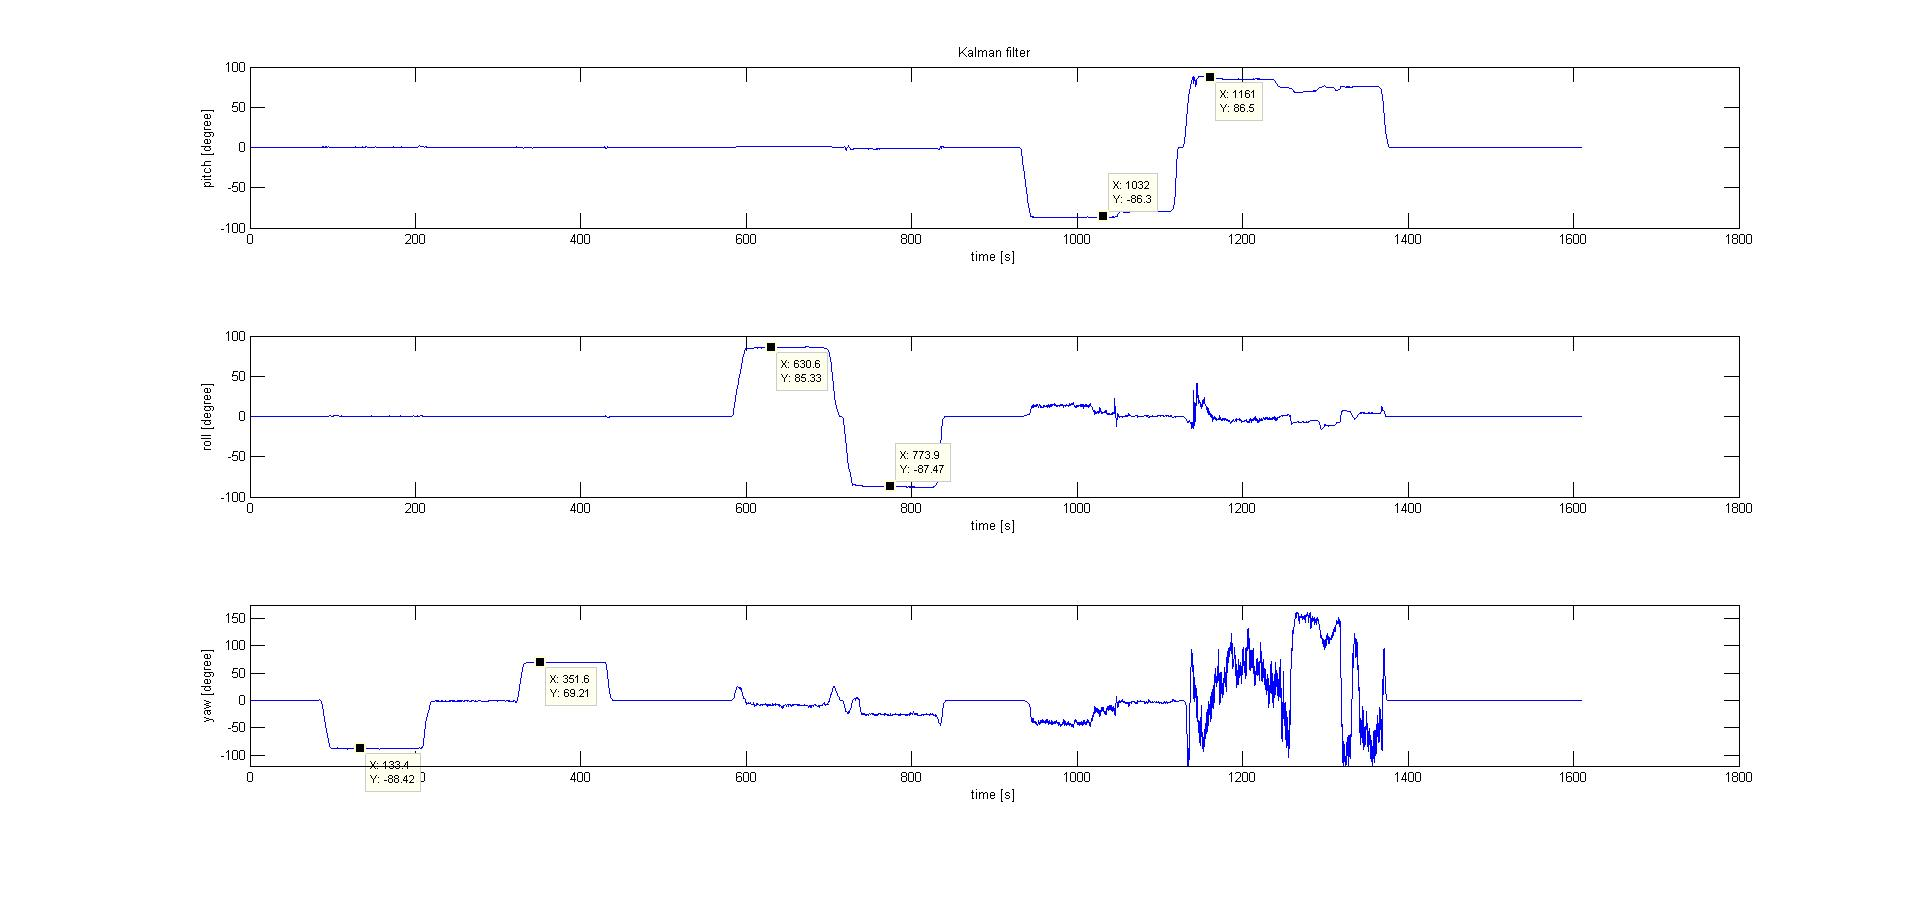
\includegraphics[width=1.0\textwidth]{fig/initial_Kalman}
	\caption{First result Kalman filter}
	\label{fig:initial_angle}
\end{figure}
\section{Magnetic sensor test}
\label{sec:MagSensTest}
As can be seen there is a problem with the yaw angle when a pitch angle is applied. This is no solution which can be used in the quadrocopter. So additional tests are made. After some time the problem was detected. Because just the yaw angle makes some problem, the main observation layed on the magnetic sensor. Figure \ref{fig:field_weak} shows the measured magnetic field.
\begin{figure}[H]
	\centering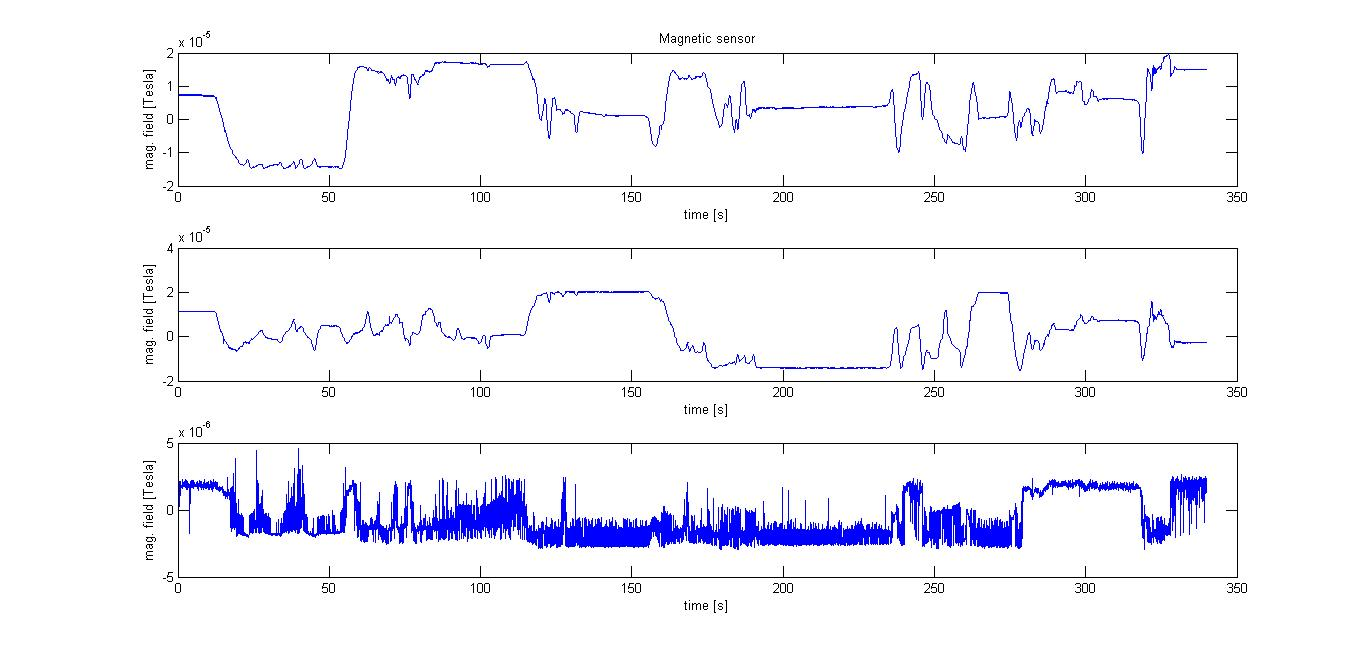
\includegraphics[width=1.0\textwidth]{fig/field_weak}
	\caption{Weak magnetic field strength}
	\label{fig:field_weak}
\end{figure}
The problem can directly be seen. The measured field strength should be nearly the same on all axis. The field strength on the x-axis and y-axis is the same. The z-axis delivers only just one tenth of the normal value. Because of that the noise on the sensor is in the same height like the signal and therefor aquiring not possible. First the position of the mounted IMU is disputed.
After changing the following sensor values of the magnetic sensor can be achieved.
\begin{figure}[H]
	\centering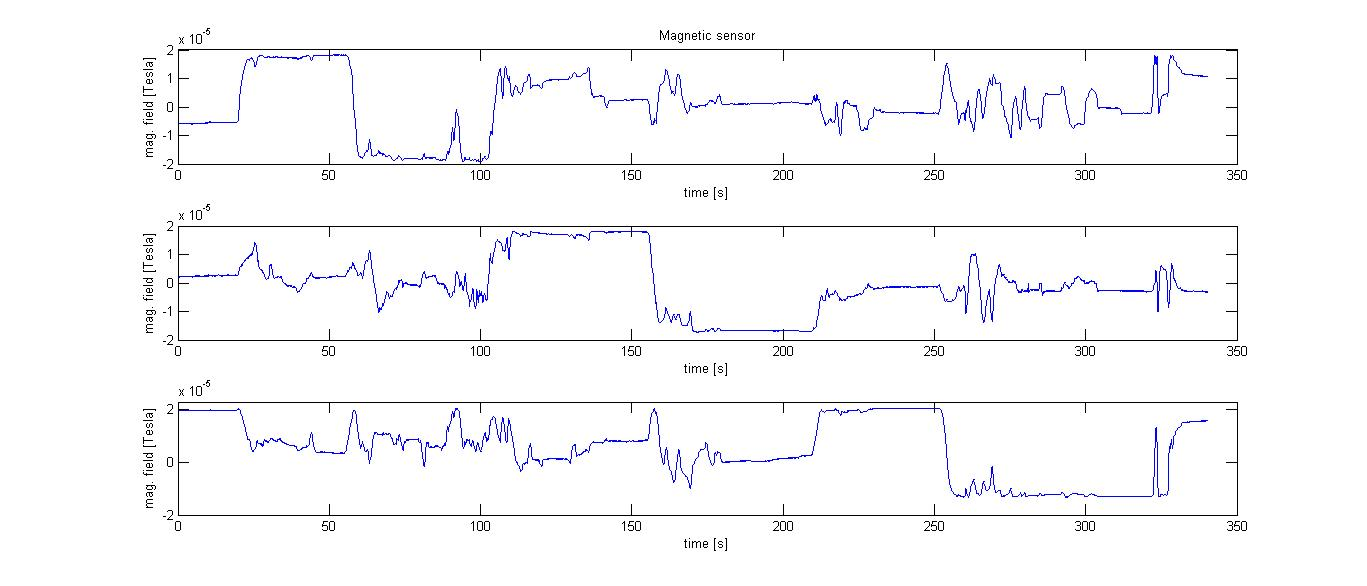
\includegraphics[width=1.0\textwidth]{fig/field_strong}
	\caption{Strong magnetic field strength}
	\label{fig:field_strong}
\end{figure}
By comparing the measurement of the initial positioning of the IMU with the new one, the strength on the z-axis is significantly higher. Also the strength on the three axis are nearly the same. So for further usage the new position is used. 

\section{Improvement magnetic sensor}
\label{sec:ImpMagSens}
The figures \ref{fig:pos_neu1} and \ref{fig:pos_neu2} shows the comparison of the mounting.
\begin{figure}[H]
	\centering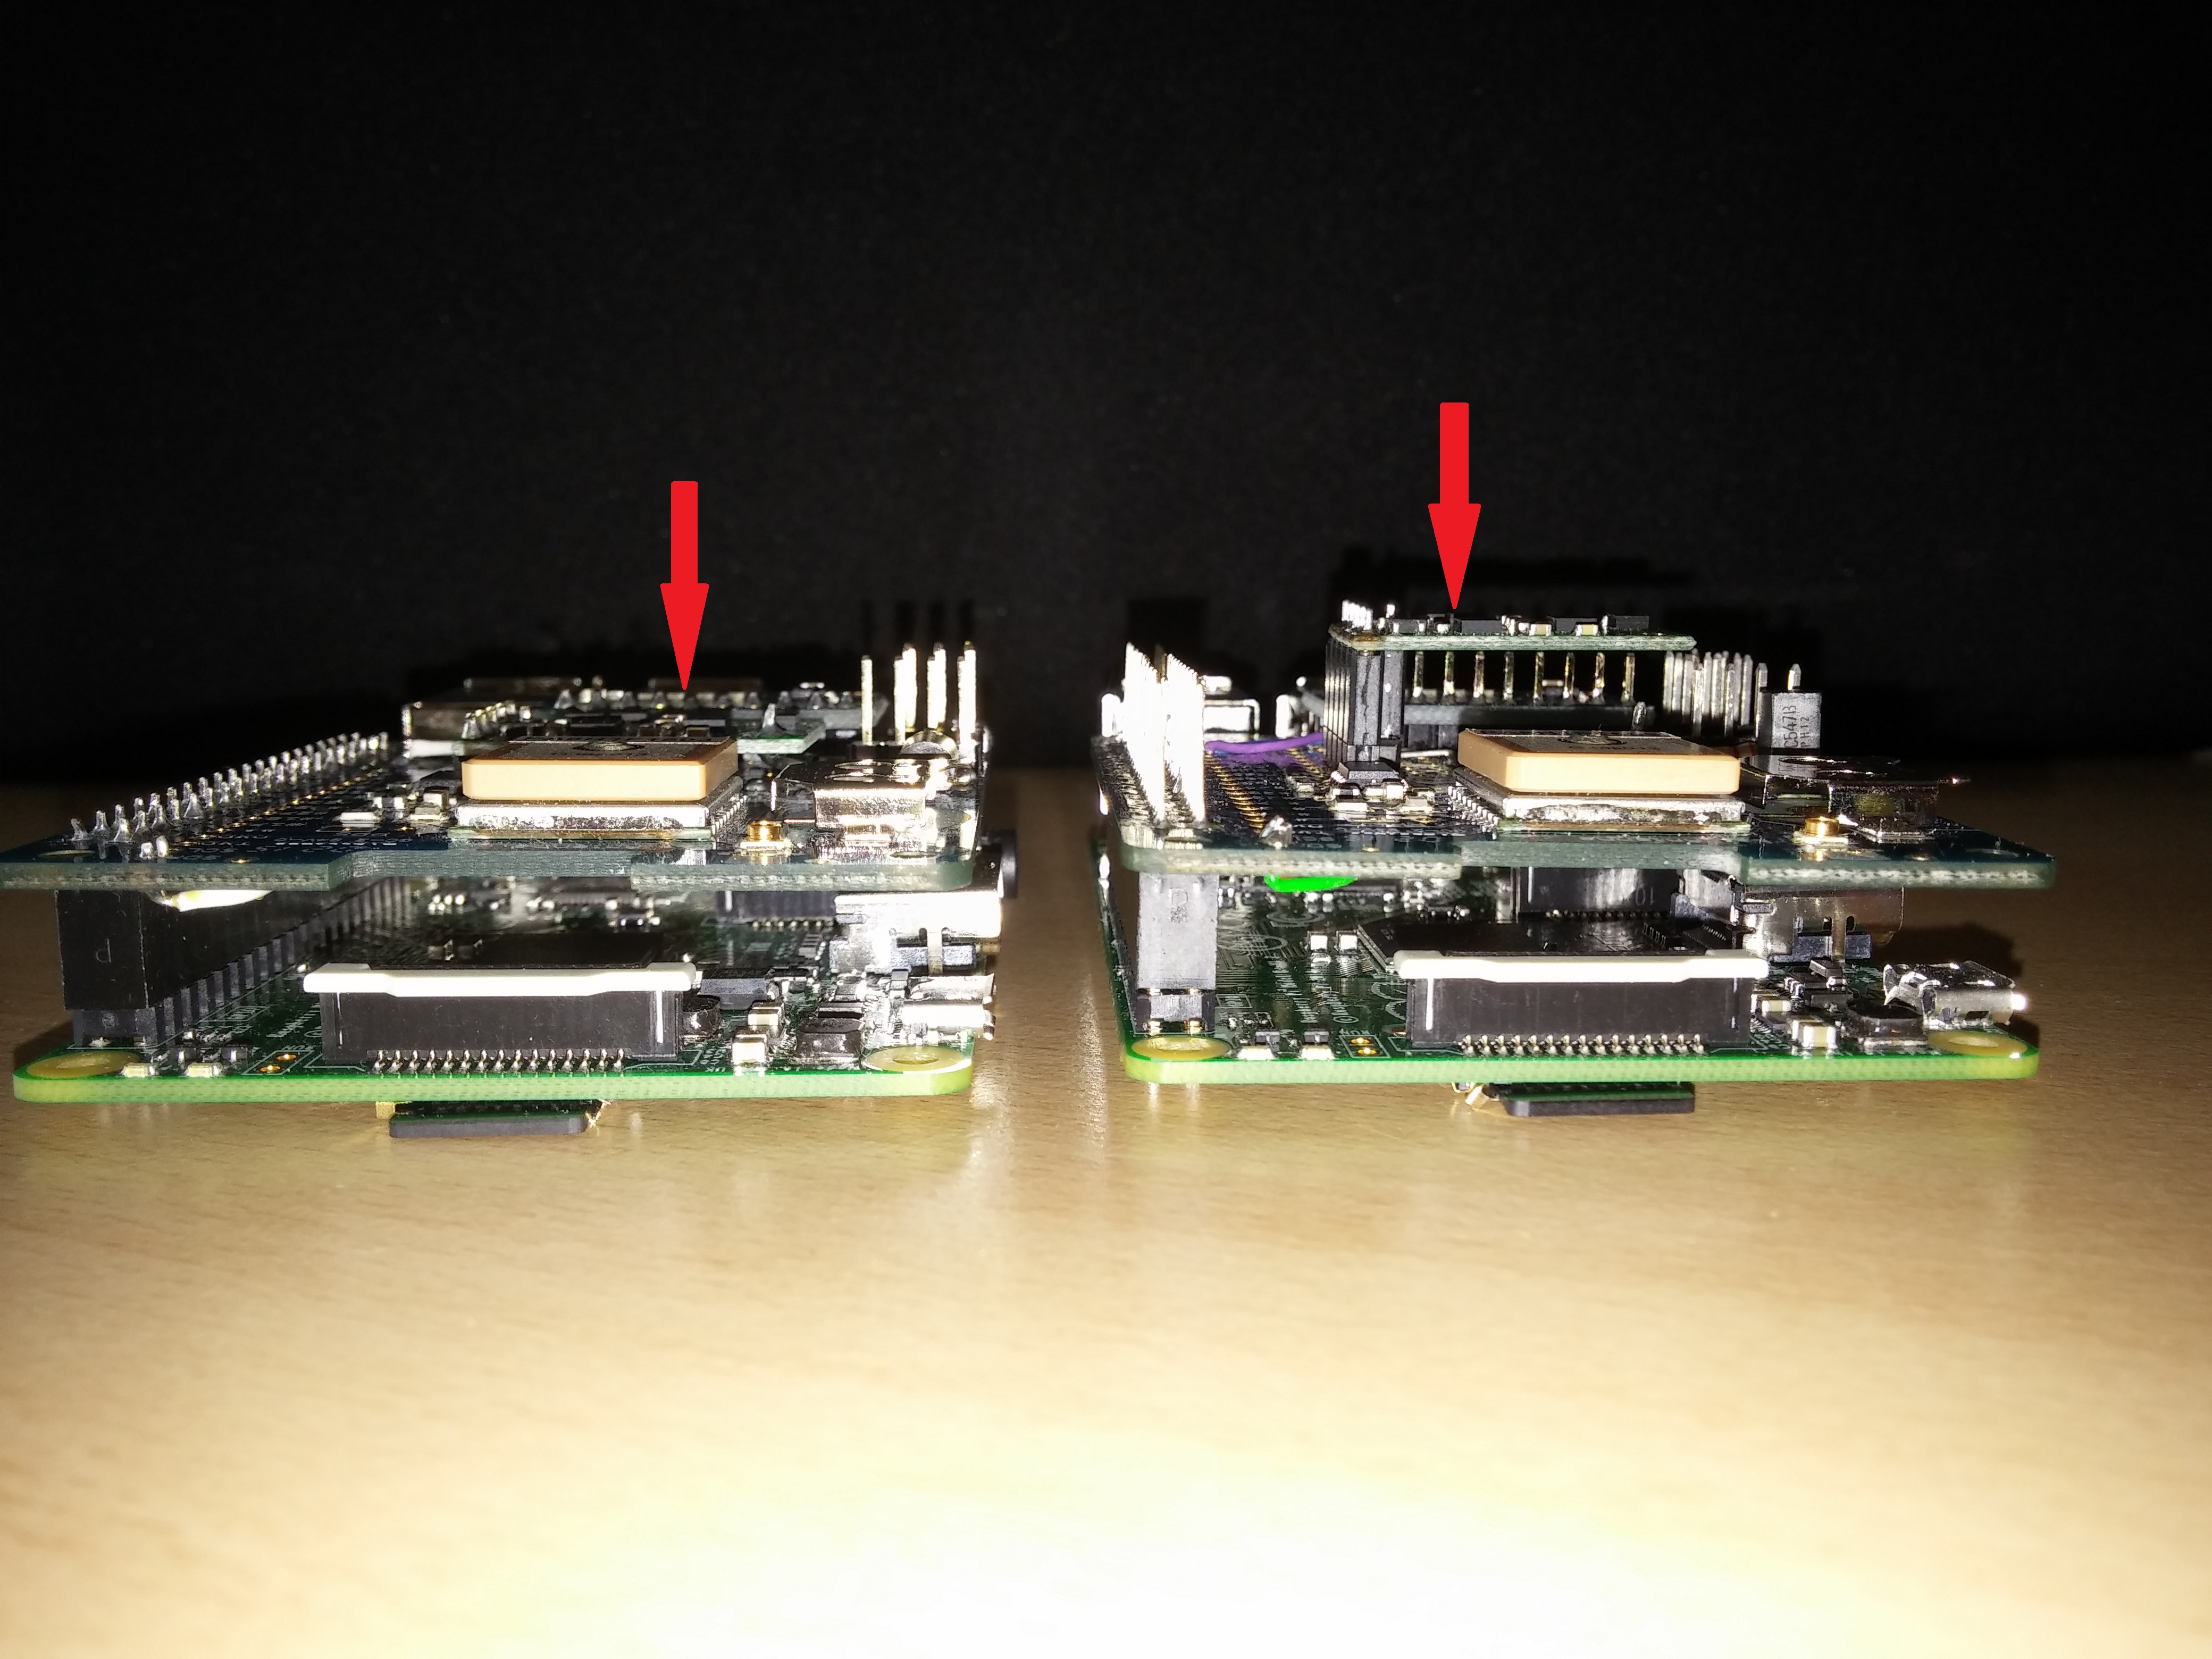
\includegraphics[width=0.6\textwidth]{fig/pos_neu1}
	\caption{New positioning of IMU 1}
	\label{fig:pos_neu1}
\end{figure}
\begin{figure}[H]
	\centering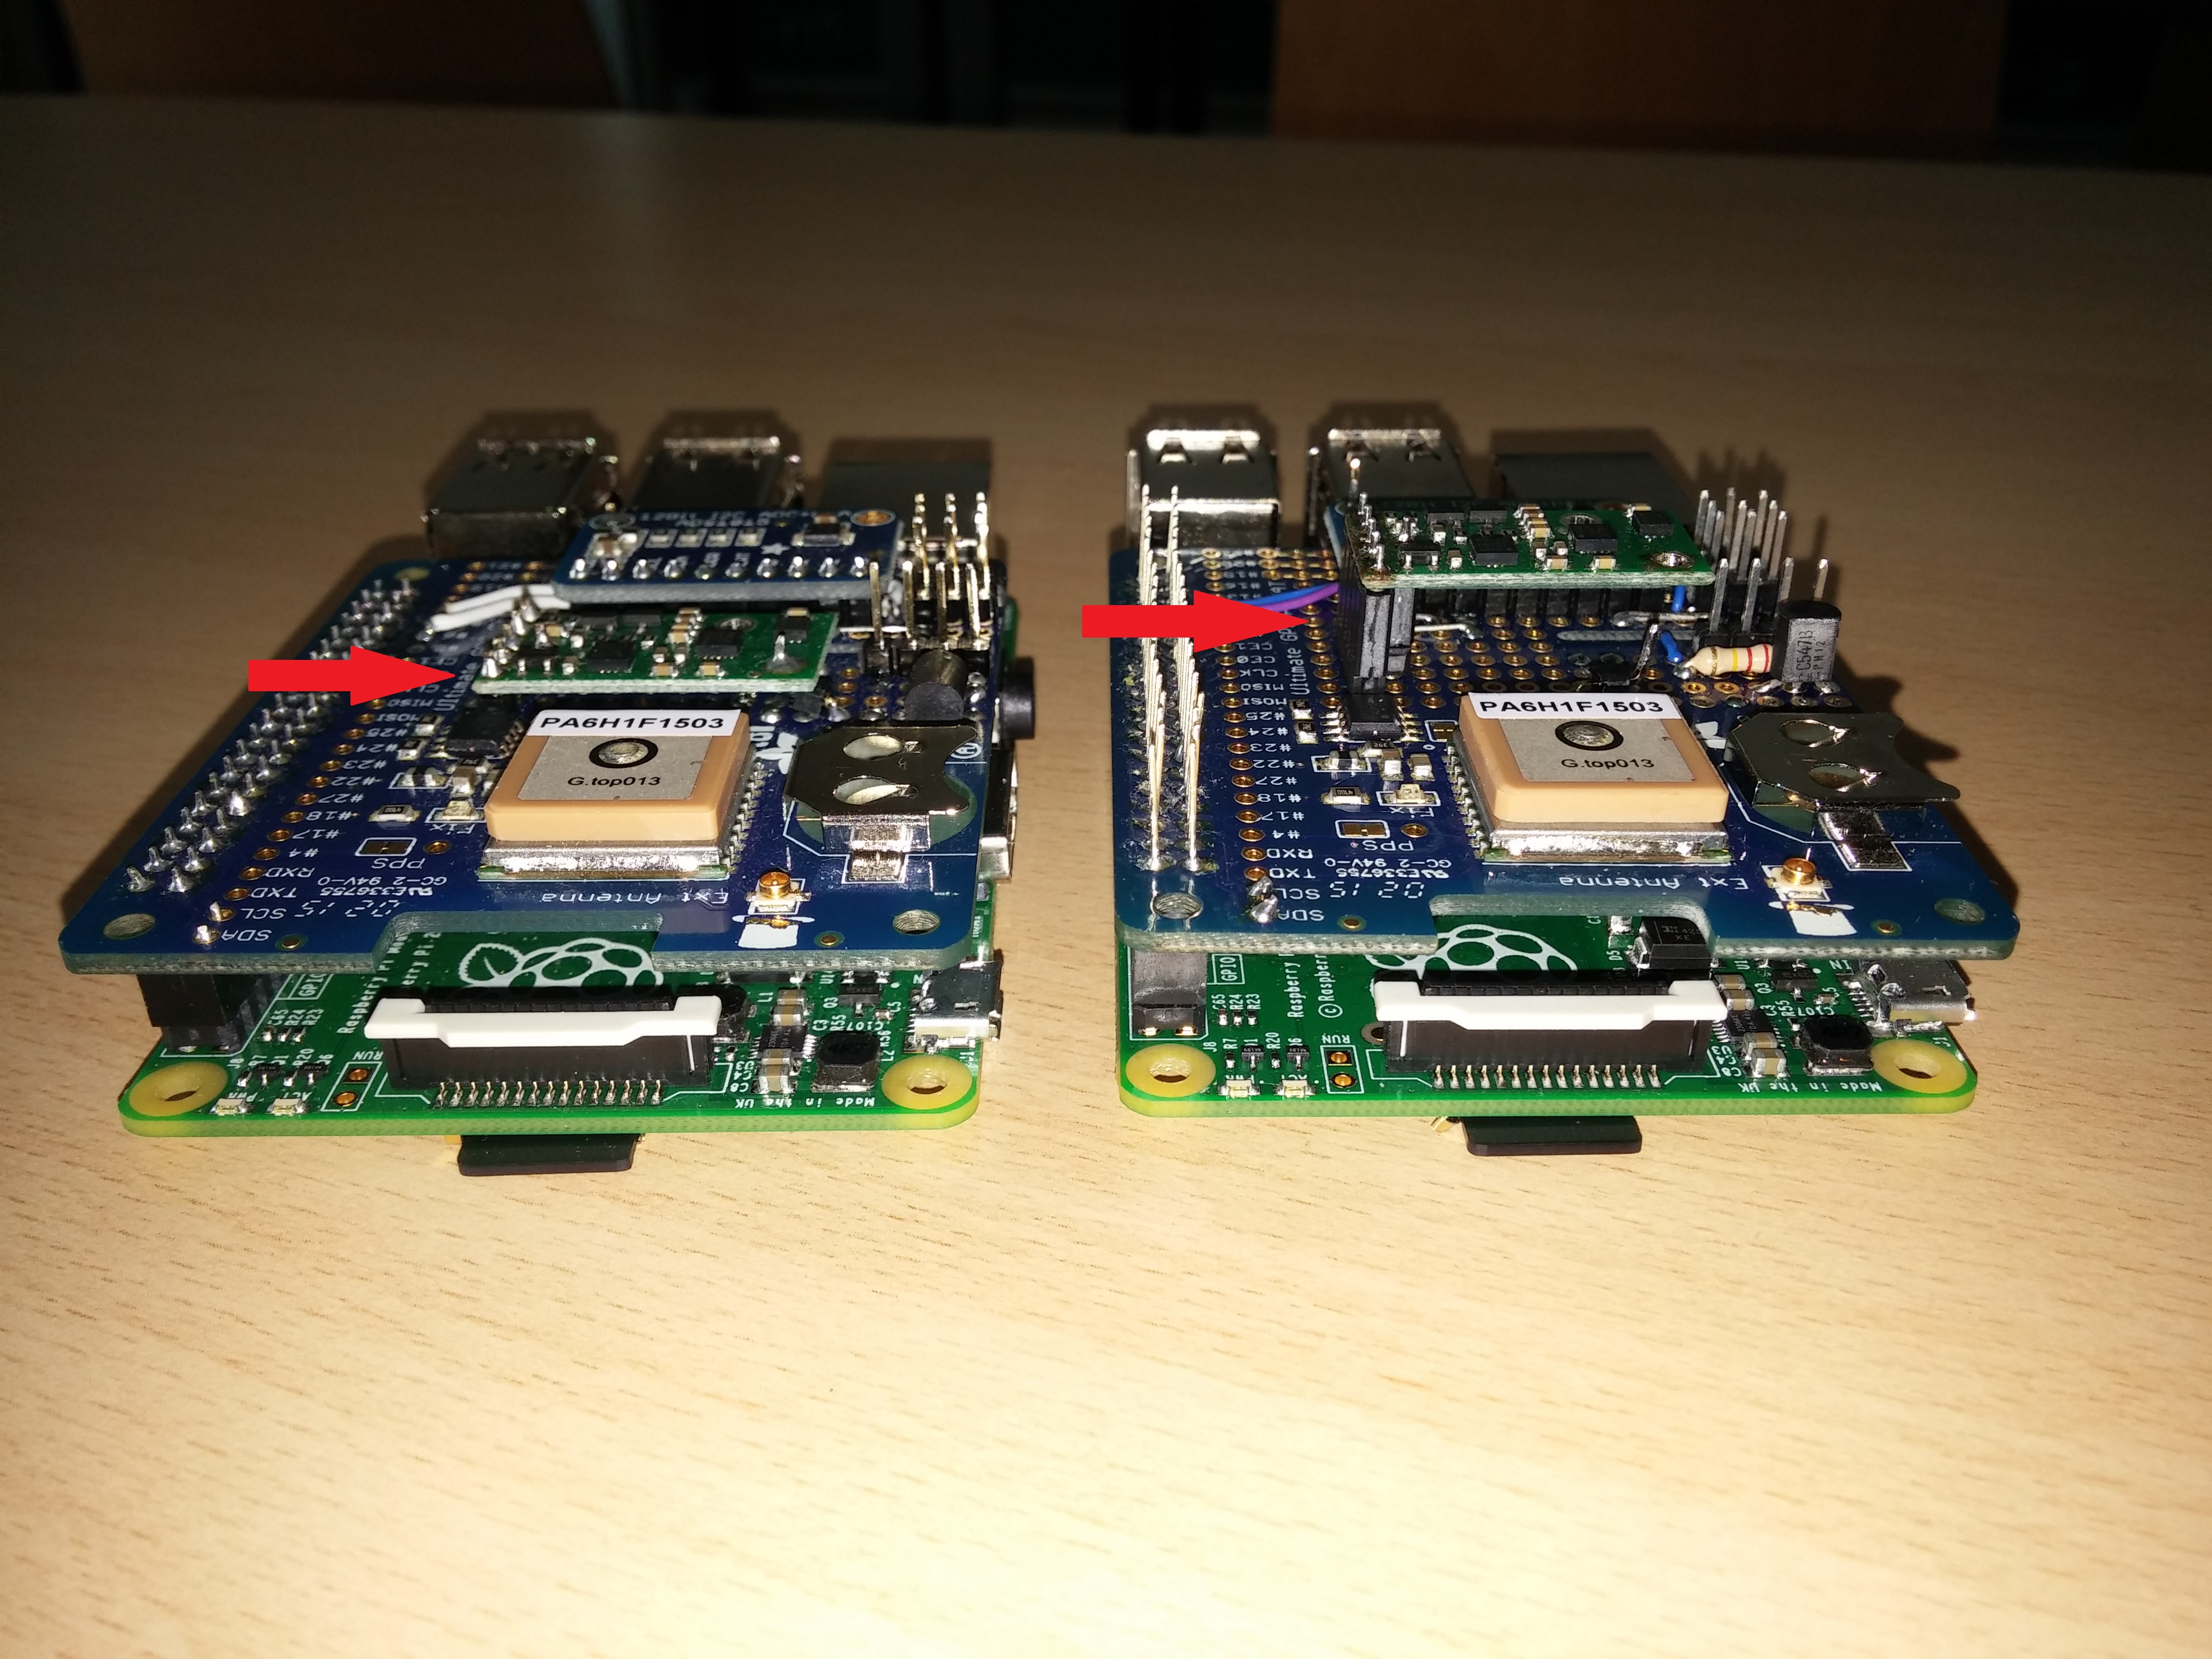
\includegraphics[width=0.6\textwidth]{fig/pos_neu2}
	\caption{New positioning of IMU 2}
	\label{fig:pos_neu2}
\end{figure}
The left PCB shows the old position and the right the new position. As can be seen just the height of the mounted IMU has to be changed. Due to the tests a distance of approximately 1cm seems to be enough. So the wiring can be kept as it is.\\
Additionally to reduce the really high influences of near metallic parts, a hard magnetic offset compensation needs to be done. Also a scaling is done. The following calculations which run in the function 'm\_sigOri\_calcAccMagAngle\_st()' are done within every step.
\begin{align}
mag_{x\_axis}=(mag_{x\_axis}-logged_{min\_x})/(logged_{max\_x}-logged_{min\_x})*2-1\\
mag_{y\_axis}=(mag_{y\_axis}-logged_{min\_y})/(logged_{min\_y}-logged_{min\_y})*2-1\\
mag_{z\_axis}=(mag_{z\_axis}-logged_{min\_z})/(logged_{min\_z}-logged_{min\_z})*2-1
\end{align}
To achieve the full range of the all three sensors the scope of Matlab can be used. The m-file which is mentioned before creates directly the header-file for the code. The improved results due to the changes which are made here can be seen in the second output of the Kalman filter and complementary filter in chapter \ref{chap:ComplementaryFilter} and \ref{chap:KalmanFilter}.
	%\chapter*{General Information}



	% % Verzeichnisse
	\tableofcontents
	\listoffigures
	\listoftables
	%\lstlistoflistings % Verzeichnis f�r Code-Listing
\end{spacing}{}
% % %%%%%% Textteil (Eigentliche Arbeit)
\mainmatter
\pagenumbering{arabic} 
%

\chapter{Introduction}
\label{ch:intro}

The very first target was to adapt a new hardware (Raspberry Pi) including a autonomous landing to the Quadrocopter from Hochschule Esslingen (HElikopter). As this was not enough work for all of us, the project was extended to include a autonomous landing, too. We were a team of 4 students who were interested in a project work with the HElikopter. We internally agreed in splitting the work in 2 parts. The other two students were more interested in developing the new hardware platform and software and we liked to care about the autonomous landing.

As we developed the autonomous landing to the new hardware, there was a slight dependence to each other.



\section{Goals}


\begin{itemize}
	\item Autonomous Landing
	\item Effective Distance measurement to ground
	\item Implementation on Raspberry Pi
\end{itemize}
% Bsp. eines Hauptteils

\chapter{Infrared Sensor}
\label{sec:infra}


We tried to establish a distance measurement with GP2Y0A60SZLF Infrared Sensor on a Pololu Carrier Board. The Measuring distance of that sensor is 10 to 150 cm. For detailed technical values, please see the sensor chapter or the datasheet.

\section{First steps}
\label{sec:infra1}

Our first action was to check, weather the sensor is working or not. So we need to active the I�C Bus on the Raspberry Pi and set up the Analog Distance Converter (ADS1011), because the Infrared Sensor provides us only a analog output.\\
We did a fast test of the sensor using python, just for checking the sensor is not broken.\\

To gather a bunch of data, we developed I�C and ADC Driver ourselfs in C.

\subsection{ADC Configuration}
\label{sec:adc_conf}

First Hex depends on Starting Conversion + the Input, which Pin to read A0-3,\\
Second Value is PGA (001)=+-4,099V and continuous Mode (0).


These three bytes are written to the ADS1015 to set the config register and start the conversion. 

  l\_writeBuf\_rg24[0] = 1;		\\
	This sets the pointer register to write two bytes to the config register
	
  l\_writeBuf\_rg24[1] = l\_mux\_ui8;   \\
	This sets the 8 MSBs of the config register (bits 15-8) to 11000011
	
  l\_writeBuf\_rg24[2] = 0x23;  		\\
	This sets the 8 LSBs of the config register (bits  7-0) to 00100011\\
	

  %First Hex is sample Rate. (001) sets to 250SPS + Comp Mode (0)\\
  %Second Hex is Comp. config. (0011) disable the comparator\\


The following table shows the Hex values in the direction from top to bottom what is needed for reading a conversion value on the specific inputs. At the empty field, there is no change compared to Input A0.

\begin{table}[H]
\begin{tabular}{|c|c|c|c|c|c|}\hline
												& Input A0 & Input A1 & Input A2 & Input A3\\ \hline
   Slave adress+RW  & 0x49 &  &  & \\ \hline
   PTR register & 0x01 &  & & \\ \hline
   %MSB Config & 0x44 & 0x54 & 0x64 & 0x74  \\ \hline
	MSB Config & 0xC2 & 0xD2 & 0xE2 & 0xF2  \\ \hline
   LSB Config  & 0x23 & & &   \\ \hline
	Slave adress+RW & 0x49 &  &  & \\ \hline
	PTR register & 0x00 &  &  & \\ \hline
	%Slave adress+RW & 0x93 & && \\ \hline
	Data from Slave & 0xXX & 0xXX & 0xXX & 0xXX\\ \hline
	Data from Slave & 0xXX & 0xXX & 0xXX & 0xXX\\ \hline
 \end{tabular}
 \caption{ADC Conversion Read}
 \label{tab:table1}
 \end{table}

MSB:\\
The first hexadecimal value is to start the conversion and depends on the Input, which Pin to read A0-3.\\
The second hexadecimal value is PGA (001)= +-4,099V and continuous Mode (0).\\

LSB:\\
The first hexadecimal value is the sample Rate. (001) sets it to 250SPS + Comp Mode (0).\\
The second hexadecimal value is the Comp. config. (0011) disables the comparator.\\


\section{Measured Values}
\label{sec:Infra2}

With our own logic getting the data from the sensor, we could store as much data we want. Now we were able to get a impression on the jitter and could thing about a good algorithm to get reliable values.

%\begin{floatingfigure}[v]{5cm}
\begin{figure}[H]
	\centering
		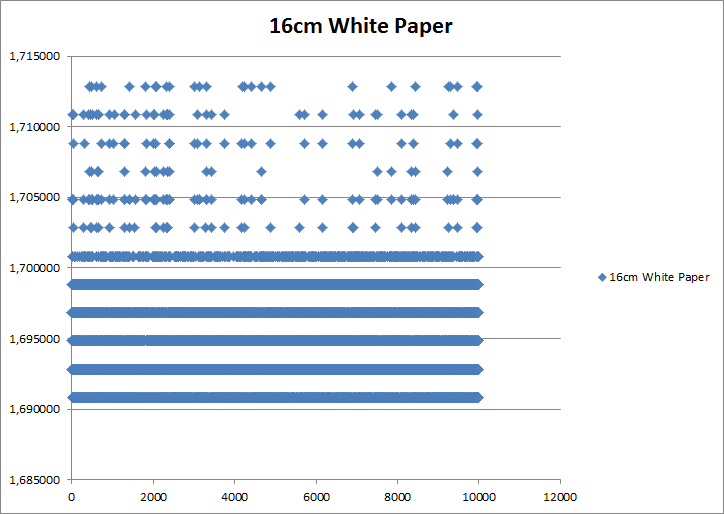
\includegraphics[width=0.8\textwidth]{fig/WhitePaper16.png}
	\label{fig:WhitePaper16}
	\caption{IR: 16 cm to white paper}
\end{figure}

Gathering 10 000 values while measuring the distance of 16cm on a white paper. We used the white paper to compare the values with them in the datasheet.\\\\

As we changed the distance and the surface, we discover a astonishing fact.\\

\begin{figure}[H]
	\centering
		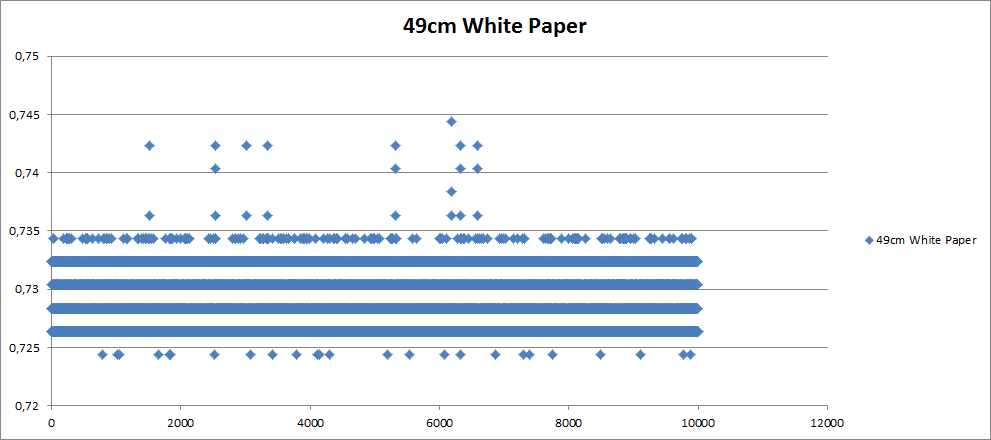
\includegraphics[width=0.8\textwidth]{fig/WhitePaper49.png}
	\label{fig:WP49}
	\caption{IR: 49 cm to white paper}
\end{figure}

Same measurement on the surface of the table:\\

\begin{figure}[H]
	\centering
		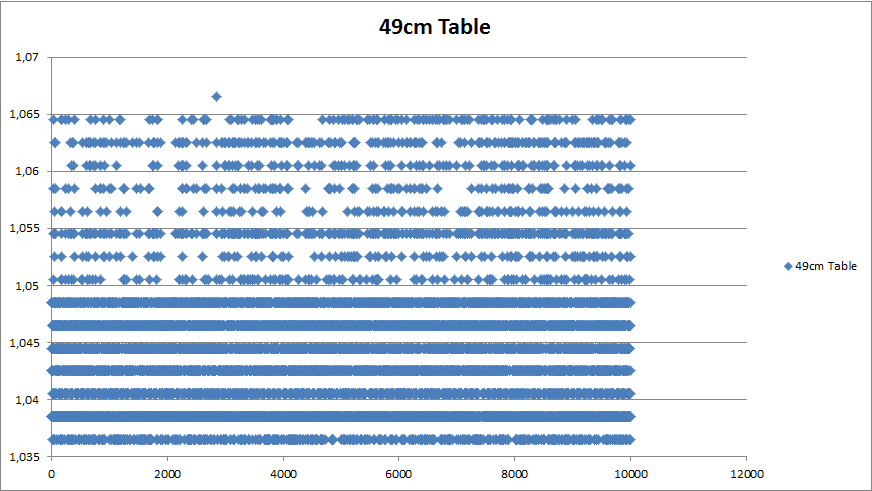
\includegraphics[width=0.8\textwidth]{fig/Table49.png}
		\caption{IR: 49 cm to table}
	\label{fig:Table49}
\end{figure}

As you see, the measurements on different surfaces are highly varying. At 49cm we got the following rough values:\\

White Paper: ~0,73 V\\
Desk Surface: ~1,42 V

\begin{figure}[H]
	\centering
		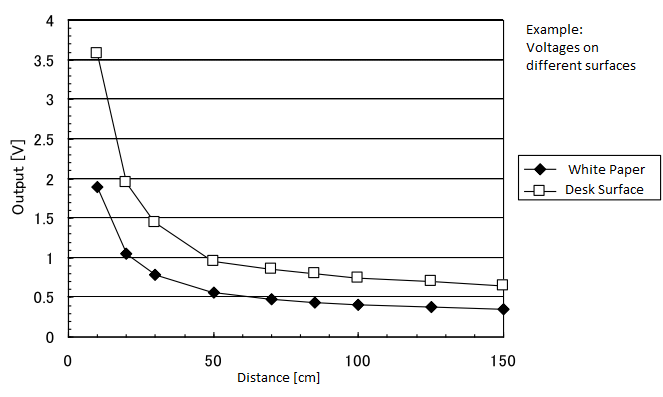
\includegraphics[width=0.8\textwidth]{fig/Surfaces_Voltages.png}
	\label{fig:WP49}
	\caption{IR: Sensor values (voltages) on different surfaces}
\end{figure}

\newpage
%\underline{2 surfaces and 2 distances}
2 Surfaces and 2 Distances:
\begin{figure}[H]
	\centering
		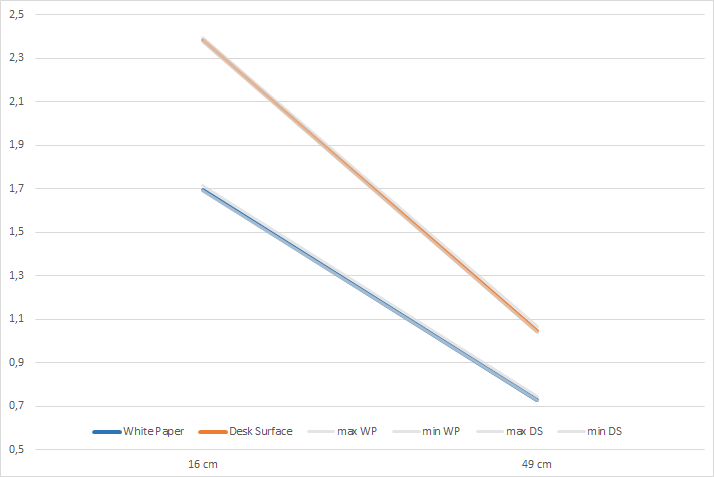
\includegraphics[width=1.0\textwidth]{fig/Surfaces_Compared.png}
	\label{fig:IR_Surf}
	\caption{IR: Compared Voltages on two surfaces}
\end{figure}

We only measured 2 different distances in order to check the functionality of the sensor. The grey lines shows the jitter which we measured. 

\section{Conclusion}
\label{sec:IRCon}

As we could not guarantee a good flying with changing surfaces, we decided to stop chasing a solution with the IR Sensor.


\chapter{Ultrasonic Distance Sensor}
\label{cha:ultra}

Our next approach was, measuring the distance with a ultrasonic distance sensor. In a meeting we agreed on using 3 ultrasonic sensor to measure the distance to ground, because a single sensor is imprecise. We hoped that a sensor fusion of 3 ultrasonics will bring us better values.\\

While searching for theses sensors, we found a relatively cheap Laser Sensor. After a short consultation, we decided to go with that one. So Ultrasonic was discarded, before start.



\chapter{LIDAR Laser Sensor}
\label{cha:laser}

LIDAR-Lite Laser Distance Sensor\\
Model LL-905-PIN-01\\

Performance\\
Range: 0-20m LED Emitter\\
Range: 0-60m Laser Emitter\\

Interfaces\\
- I$^2$C\\
- PWM\\

For detailed technical values, please see the sensor chapter or the datasheet.\\

\section{Connecting the sensor with I$^2$C}
\label{sec:lascon}

Because there is no proper input for a PWM signal, we used the I$^2$C Bus to connect the laser sensor. As the sensor does not support fast I$^2$C mode, which we need, we decided to use the second I$^2$C on the Raspberry Pi. This bus is orginally located on the camera port with an FPC (flexible printed circuit) Connector. We managed it to redirect it to the normal Pins on the board. See Chapter xxxxxx.

\section{First steps}
\label{sec:lasfirst}

Quick Start Guide 

1.  Make Power and I2C Data Connections as per J1 connector pin out diagram.  Pins 2 \& 3 are optional connections and not required. \\
2.  Initialization:  Apply Power to the Module. The sensor operates at 4.75-5.5V DC Nominal, Maximum 6V DC.\\
3.  Measurement: Write register 0x00 with value 0x04 (This performs a DC stabilization cycle, Signal Acquisition, Data processing). Refer to the section "`I2C Protocol Summary"' in this manual for more information about I2C Communications.\\
4.  Periodically poll the unit and wait until an ACK is received. The unit responds to read or write requests with a NACK when the sensor is busy processing a command or performing a measurement. 
(Optionally, wait approx. 20 milliseconds after acquisition and then proceed to read of high and low bytes) \\
5.  Read:  register 0x0f, returns the upper 8 bits of distance in cm, register 0x10, returns the lower 8 bits of 
distance in cm.  (Optionally a 2-Byte read starting at 0x8f can be done) 


\section{Measured Values}
\label{sec:lasvalues}

\section{conclusion}
\label{sec:lasconlu}



   
\chapter{I$^2$C Configuration}
\label{chap:I2C}
This document describes all necessary steps to get the two I$^2$C Busses of the Raspberry Pi (Model B+) up and running. Because of different operating modes of the devices using the I$^2$C-Bus the usage of both busses is necessary.\newline\newline
\textbf{HINT: These steps are not necessary if you install the Rasbian Image of the Projekt. There everything should be configured.}\newline


\section{raspi-config}
\label{sec:raspiconfig}
Enable I$^2$C using raspi-config utility.\\\\
From the command line type:\\\\
\ttfamily \textbf{sudo raspi-config}\\\\
\normalfont This will open the raspi-config utility.

\begin{figure}[H]
	\centering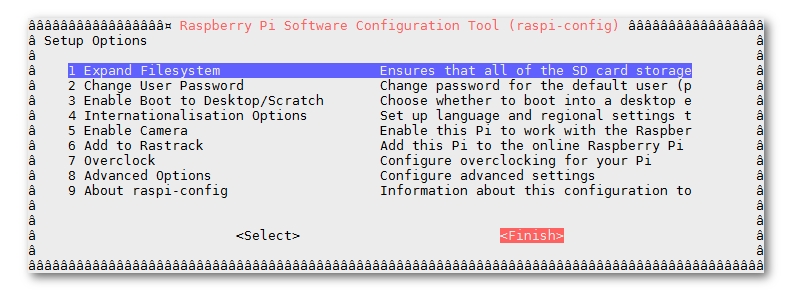
\includegraphics[width=\textwidth]{fig/raspi_config}
	\caption{raspi-config}
	\label{fig:raspiconfig}
\end{figure}

\newpage
\textbf{Now complete the following steps:}\\\\
Select: "8 - Advanced Options"\\
Select: "A7 - I$^2$C"\\
Select: "Yes"\\
The Screen will ask if you want the interface to be enabled:\\
Select: "Yes"\\
Select: "OK"\\
The Screen will ask if you want the module to be loaded by default:\\
Select: "Yes"\\
The Screen will state the module will be loaded by default:\\
Select: "OK"\\
Select "Finish" to return to the command line \\
When you next reboot the I$^2$C module will be loaded.\\


\section{Module File}
\label{sec:modulefile}
Next we need to edit manually the modules file using:\\
\ttfamily \textbf{sudo nano /etc/modules}\\
\normalfont and add the following lines:\\
\ttfamily \textbf{i2c-bcm2708\\
									i2c-dev}\\
\normalfont									
Use CTRL-X, then Y, then RETURN to save the file and exit.								





\section{I$^2$CTools}
\label{sec:I2Ctools}

For hardware monitoring, device identification, and troubleshooting we install "i2c-tools".\\\\
\ttfamily \textbf{sudo apt-get update\\
									sudo apt-get install i2c-tools}\\\\
\normalfont
Now shutdown your system, disconnect the power to your Pi and you are ready to connect your I$^2$C-hardware.\\									


\section{Test I$^2$C-1}
\label{sec:testi2c1}

\textbf{Check if I$^2$C is enabled:}\\\\
When you power up or reboot your Pi you can check the I$^2$C module is running by using the following command:\\
\ttfamily \textbf{lsmod $|$ grep i2c\_}\\
\normalfont
That will list all the modules starting with "i2c\_". If it lists "i2c\_bcm2708" then the module is running correctly.\\\\

\textbf{Testing Hardware:}\\
Once you've connected your hardware double check the wiring. Make sure 5V is going to the correct pins and you've got not short circuits. Power up the Pi and wait for it to boot.\\
Then type the following command:\\\\
\ttfamily \textbf{sudo i2cdetect -y 1}\\\\
\normalfont 
With e.g. a sensor connected the output looks e.g. like this:\\

\ttfamily
 \quad\quad  0  1  2  3  4  5  6  7  8  9  a  b  c  d  e  f \\
00:\qquad\quad\quad-- -- -- -- -- -- -- -- -- -- -- -- -- \\
10: -- -- -- -- -- -- -- -- -- -- -- -- -- -- -- -- \\
20: -- -- -- -- -- -- -- -- -- -- -- -- -- -- -- -- \\
30: -- -- -- -- -- -- -- -- -- -- -- -- -- -- -- -- \\
40: -- -- -- -- -- -- -- -- -- -- -- -- -- -- -- -- \\
50: -- -- -- -- -- -- -- -- -- -- -- -- -- -- -- -- \\
60: -- -- 62 -- -- -- -- -- -- -- -- -- -- -- -- -- \\
70: -- -- -- -- -- -- -- -- \\\\
\normalfont

This shows that one device is connected and its address is 0x62.\\ 


\newpage

\section{Set up I$^2$C-0}
\label{sec:setupi2c0}


In normal configuration the second I$^2$C-Bus of the Raspberry Pi is set up as two of the output pins of the DSI Display Connector resp. the CSI Camera Connector.\\
To make the setup of the quadrocopter as easy as possible and with respect to the weight and soldering/cabling these output pins were redirecteed to two of the 40 pins of the GPIO Header.\\

This gets done by useage of a Python-script (see below) which gets excecuted while booting the system. To get this configuration running two additional files need to be edited.\\\\
In "/boot/cmdline.txt"\\
\ttfamily bcm2708.vc\_i2c\_override=1 \\
\normalfont has to be added\\
in "/etc/modprobe.d/i2c\_o\_enable.conf"\\
\ttfamily{blacklist snd\_soc\_tas5713} \\
\normalfont has to be added.\\

After this the GPIO port 27 is configured as SDA0 and the GPIO port 28 as SCL0.

\begin{figure}[H]
	\centering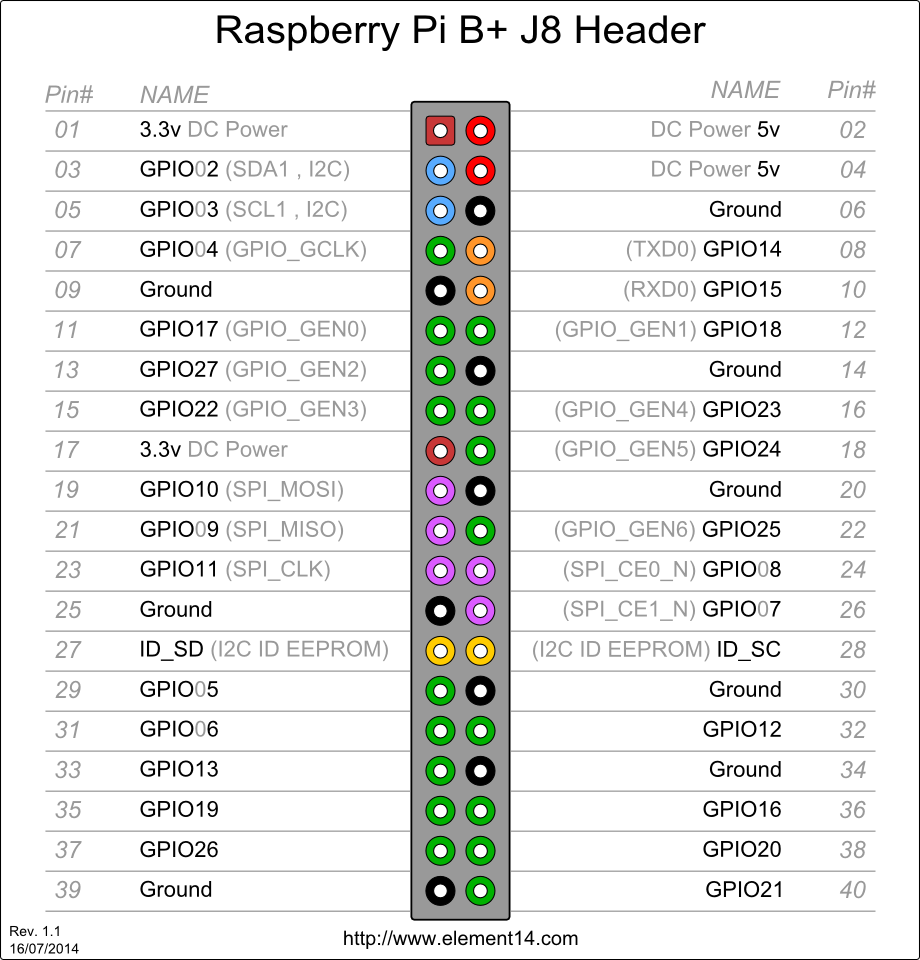
\includegraphics[width=0.5\textwidth]{fig/gpios}
	\caption{GPIOs \footnotemark}
	\label{fig:gpios}
\end{figure}
\footnotetext{\url{http://www.element14.com/community/servlet/JiveServlet/previewBody/68203-102-6-294412/GPIO.png}}
\newpage


\lstinputlisting[language=Python, basicstyle=\tiny, caption=I$^2$C0 Port-Configuration]{add_files/I2C0_Config_OS.py}





% Bsp. eines Hauptteils

\chapter{Functions in C}
\label{ch:functions}

These chapter is about the C-Code we developed to work via Raspberry Pi with the sensors.


\section{I$^2$C}

%-------------  write I2C 0 ---------------------%
\begin{lstlisting}[language=C, basicstyle=\small, caption=Write on I2C-1]
unsigned int g_lldI2c_WriteI2c_bl(unsigned char, const unsigned char*, unsigned int);
\end{lstlisting}


\begin{tabular}{lll}
Parameter: & unsigned char & slave address of device\\
					 & const unsigned char* & buffer with data to write\\
					 & unsigned int & number of bytes to write\\
					 &	\\
Return: & unsigned int & error detection, 0=OK 1=failure\\
							&&\\
Description: & \multicolumn{2}{l}{function to write several data on the I2C-1 Bus of the Raspberry PI}\\
\end{tabular}
\\

%-------------  read I2C 0 ---------------------%

\begin{lstlisting}[language=C, basicstyle=\small, caption=Read from I2C-1]
unsigned int g_lldI2c_ReadI2c_bl(unsigned char, const unsigned char*, unsigned int);
\end{lstlisting}

\begin{tabular}{lll}
Parameter: & unsigned char & slave address of device\\
					 & const unsigned char* & array to store read data\\
					 & unsigned int & number of bytes to read\\
					 &	\\
Return: & unsigned int & error detection, 0=OK 1=failure\\
							&&\\
Description: & \multicolumn{2}{l}{function to read several data on the I2C-1 Bus of the Raspberry PI}\\
\end{tabular}
\\

%-------------  write I2C 1 ---------------------%

\begin{lstlisting}[language=C, basicstyle=\small, caption=Write on I2C-0]
unsigned int g_lldI2c_WriteI2c0_bl(unsigned char, const unsigned char*, unsigned int);
\end{lstlisting}


\begin{tabular}{lll}
Parameter: & unsigned char & slave address of device\\
					 & const unsigned char* & buffer with data to write\\
					 & unsigned int & number of bytes to write\\
					 &	\\
Return: & unsigned int & error detection, 0=OK 1=failure\\
							&&\\
Description: & \multicolumn{2}{l}{function to write several data on the I2C-0 Bus of the Raspberry PI}\\
\end{tabular}
\\


%-------------  read I2C 1 ---------------------%

\begin{lstlisting}[language=C, basicstyle=\small, caption=Read from I2C-0]
unsigned int g_lldI2c_ReadI2c0_bl(unsigned char, const unsigned char*, unsigned int);
\end{lstlisting}

\begin{tabular}{lll}
Parameter: & unsigned char & slave address of device\\
					 & const unsigned char* & array to store read data\\
					 & unsigned int & number of bytes to read\\
					 &	\\
Return: & unsigned int & error detection, 0=OK 1=failure\\
							&&\\
Description: & \multicolumn{2}{l}{function to read several data on the I2C-0 Bus of the Raspberry PI}\\
\end{tabular}
\\





\subsection{Configuration}

$\#include <linux/i2c-dev.h>$ is doing the (local) device handling. We only use the slave address to communicate with the connected devices. Read or write commands are provided by fcntl.h.

\subsection{I$^2$C Write}

Writes the number of stated bytes from the write buffer with the "write" command to the chosen I$^2$c-device, depending on called function.

\subsection{I$^2$C Read}

Reads the number of stated bytes from the read buffer with the "read" command from the chosen I$^2$c-device, depending on called function.



\newpage
\section{Analog-Digital-Converter (ADC)}

\begin{lstlisting}[language=C, basicstyle=\small, caption=Read from ADC]
float g_halADC_get_ui16(unsigned char );
\end{lstlisting}


\begin{tabular}{lll}
Parameter: & unsigned char & A0-A3 input selection\\
					 &	\\
Return: & float & converted analog values\\
							&&\\
Description: & \multicolumn{2}{l}{Interface to read ADS1015 (ADC)}\\
\end{tabular}
\\


\subsection{Configuration}

Sensor Board Name: Pololu ADS1015\\
Sensor Name: GP2Y0A60SZLF\\

l\_mux\_ui8 = 0xC2;\\
" C "\textsubscript{16}:\\
The first Hex-Value depends on Starting Conversion + the Input, which Pin to read A0-3

" 2 "\textsubscript{16}: \\
The second Value is PGA (001)=+-4,099V and continuous Mode (0)\\


These three bytes are written to the ADS1015 to set the config register and start the conversion 

l\_writeBuf\_rg24[0] = 1;		\\ 
This sets the pointer register to write the following two bytes to the config register

l\_writeBuf\_rg24[1] = l\_mux\_ui8;   	\\ 
This sets the 8 MSBs of the config register (bits 15-8) to 11000011

l\_writeBuf\_rg24[2] = 0x23;  		\\ 
This sets the 8 LSBs of the config register (bits  7-0) to 00100011\\   


" 2 "\textsubscript{16}:\\
  // First Hex is sample Rate. (001) sets to 250SPS + Comp Mode (0)
	
" 3 "\textsubscript{16}:\\
  // Second Hex is Comp. config. (0011) disable the comparator
	
	
	
The l\_writeBuf\_rg24 is written to the configuration register of the ADC. After that, we can read the converted analog values from the chosen input.



\subsection{ADC Read}

To read a converted analog value, you need to set the pointer register to 0.\\

When the pointer register is set to 0 this signals that the converted analog value should be provided. You will get the these values when performing a i$^2$c-read command the next time. This value is 16 Bit large and will be calculated as a float-value, depending on the resolution which is adjusted.






\section{Infrared Sensor}

\begin{lstlisting}[language=C, basicstyle=\small, caption=Read Infrared]
float g_halADC_get_ui16(unsigned char );
\end{lstlisting}

\begin{tabular}{lll}
Parameter: & char & select Input on which IR is connected\\
					 &	\\
Return: & float & Voltage from Sensor\\
							&&\\
Description: & \multicolumn{2}{l}{Since our IR Sensor only provides analog output, we need to use the ADC}\\
\end{tabular}
\\



\subsection{Configuration}

There is no configuration of the Infrared sensor needed.

\subsection{Read Sensor Values}

We get the analog values with the ADC-Function.





\section{LIDAR-Lite Laser Sensor}








\begin{lstlisting}[language=C, basicstyle=\small, caption=get Laser Distance]
double g_LIDAR_getDistance_f64(void);
\end{lstlisting}

\begin{tabular}{lll}
Parameter: & void & \\
					 &	\\
Return: & double & distance in meter\\
							&&\\
Description: & \multicolumn{2}{l}{returns calculated distance value in meters}\\
\end{tabular}
\\

\begin{lstlisting}[language=C, basicstyle=\small, caption=trigger Laser measurement]
int g_LIDAR_readDistanceFromI2C_i32(void);
\end{lstlisting}

\begin{tabular}{lll}
Parameter: & void & \\
					 &	\\
Return: & int & error detection, 0=OK -1=failure\\
							&&\\
Description: & \multicolumn{2}{l}{triggers a measurement and stores the result}\\
\end{tabular}
\\


\subsection{Configuration}

Trigger Measurement of Distance (DC stabilization cycle, Signal Acquisition, DataProcessing)\\

First Config Byte: 0x00;\\
Representation of configuration register 0x00 of the laser sensor.\\
Second Config Byte: 0x04;\\
Take acquisition and correlation processing with DC correction\\

Set Reg 0x8f as Output-Register to read a two-byte value which gives the distance in cm.\\

\subsection{Read Sensor Values}

Read two-byte distance in cm from register 0x8f. This value is stored as a decimal value in cm.\\
Alternative you can read the high-byte of the measured value from register 0x0f and the low-byte from register 0x10.\\


%\chapter{Ergebnisse}
%\label{sec:ergeb}
%\enquote{Neuigkeiten} Messergebnisse
%
%\section{Literaturverweise}
%\label{sec:real-literatur}
%
%Verweise im Text: \cite{doc:stz} und \cite{doc:gun}.



% % Preamble BEGINN %%%%%%%%%%%%%%%%%%%%%%%%%%%%%%%%%%%%%%%%%%%%%%%%%%%%%%%%%

%%% Preamble (Dokumentenklasse)
% ------------------------------------------------------------------------
% LaTeX - Preambel ******************************************************
% ------------------------------------------------------------------------
% Dokumentklasse (Koma Script)
% ------------------------------------------------------------------------
% basiernd auf www.matthiaspospiech.de/latex/vorlagen Diplomarbeit kompakt
% ========================================================================
\documentclass[%
   %draft,            % Entwurfsstadium
   final,             % fertiges Dokument
   12pt,              % Schriftgroesse der Grundschrift
   bigheadings,       % gro�e �berschriften
   ngerman,           % wird an andere Pakete weitergereicht
   a4paper,           % Papierformat
   BCOR5mm,          % Bindekorrektur: Zus�tzlicher Rand auf der Innenseite
   DIV14,            % Seitengr��e (siehe Koma Skript Dokumentation !)
   1.1headlines,     % Zeilenanzahl der Kopfzeilen
   pagesize,         % Schreibt die Papiergroesse in die Datei.
   oneside,          % Einseitiges Layout
%   twoside,          % Zweiseitiges Layout
   openright,        % Kapitel beginnen immer auf der rechten Seite
   titlepage,        % Titel als einzelne Seite ('titlepage' Umgebung)  
   headsepline,      % Linie unter Kolumnentitel ()
%   plainheadsepline, % Linie unter Kolumnentitel () plain Seitenstil
   nochapterprefix,  % keine Ausgabe von 'Kapitel:'
   bibtotoc,         % Bibliographie ins TOC
%	bibtotocnumbered, % Bibliographie ins TOC mit Kapitelnummer
   tocindent,        % eingereuckte Gliederung
   listsindent,      % eingereuckte LOT, LOF
   pointlessnumbers, % �berschriftnummerierung ohne Punkt, siehe DUDEN !
   cleardoubleempty, % Leere linke Seite bei Zweiseitenlayout vor Kapitel
   fleqn,            % Formeln werden linksbuendig angezeigt
%   parindent,        % Absatz mit Einzug (Standard)
   halfparskip,      % Absatz halbe Zeile Abstand
%   parskip,          % Absatz ganze Zeile Abstand
]{scrbook}%     Klassen: scrartcl, scrreprt, scrbook


%%% Alle Namen usw. im Titel und im hyperref-Paket
% ------------------------------------------------------------------------
% LaTeX - Preambel ******************************************************
% ------------------------------------------------------------------------
% pre-work
% ========================================================================
% % ToDo kennzeichnen
\newcommand{\workTodo}[1]{\textcolor{red}{todo: #1}}

% % F�r Datum und Zeit in Fusszeile
% % !!!Inhalt bei Fertigstellung der Arbeit l�schen
\newcommand{\workMarkDateTime}{\today{}  }

% % Alle Namen werden im Titel und im hyperref-Paket eingetragen
% % !!! Ueberall f�r <Wert> das Entsprechende eintragen

 % <Typ> Studienarbeit, Dipolmarbeit, Studienarbeit oder Bachlor-Abschlussarbeit
\newcommand{\workTyp}{Team Project\xspace}

 % <Titel> der Arbeit
\newcommand{\workTitel}{Quadrocopter}

 % <Studiengang> z.B. Kommunikationstechnik
\newcommand{\workStudiengang}{ASM-SB \xspace}

% <Semester> mit Jahr z.B. Sommersemester 2008  
\newcommand{\workSemester}{ASM2\xspace}

% <Name> des Studenten
\newcommand{\workNameStudentOne}{Oliver Breuning\xspace}
\newcommand{\workNameStudentTwo}{Martin Brodbeck\xspace}
\newcommand{\workNameStudentThree}{J\"urgen Schmidt\xspace}
\newcommand{\workNameStudentFour}{Phillip Woditsch\xspace}

% <Pruefer> Name des pr�fenden (betreuenden) Professor an der Hochschule
\newcommand{\workPruefer}{Prof. Dr. J\"org Friedrich\xspace} 


% %%% Nur bei Abschluss-Arbeiten

% <Datum> der Abgabe der Arbeit (Eidesstatliche Erkl�rung)
\newcommand{\workDatum}{\today\xspace}

% <Zweitpr�fer>
\newcommand{\workZweitPruefer}{\workTodo{<Zweitpr�fer>}\xspace}

% <Zeitraum>
\newcommand{\workZeitraum}{Summersemester 2015\xspace}


% %%% Nur bei Industrie-Arbeiten:

% <Firma>
\newcommand{\workFirma}{\workTodo{<Firma>}\xspace}

% <Betreuer in der Firma>
\newcommand{\workBetreuer}{\workTodo{<Betreuer in der Firma>}\xspace}

% Firmenlogo Name hier anpassen, Gr��e (wenn m�glich) nicht �ndern
%\newcommand{\workFirmenLogo}{
\includegraphics[width=5cm]{fig/aa-titel/Bosch_4C_S}} 


%%% Preamble (Pakete)
% ------------------------------------------------------------------------
% LaTeX - Preambel ******************************************************
% ------------------------------------------------------------------------
% Packages
% ------------------------------------------------------------------------
% basiernd auf www.matthiaspospiech.de/latex/vorlagen Diplomarbeit kompakt
% ========================================================================

% Inhalt:
% 1. Einige Pakete muessen unbedingt vor allen anderen geladen werden
% 2. Fonts Fonts Fonts
% 3. Math Packages
% 4. Symbole
% 5. text related packages
% 6. Pakete zum Zitieren
% 7. PDF related packages
% 8. Tables (Tabular)
% 9. figures and placement
% 10. verbatim packages
% 11. science packages
% 12. layout packages

% ~~~~~~~~~~~~~~~~~~~~~~~~~~~~~~~~~~~~~~~~~~~~~~~~~~~~~~~~~~~~~~~~~~~~~~~~
% Encoding der Dateien (sonst funktionieren Umlaute nicht)
% Empfohlen latin1, da einige Pakete mit utf8 Zeichen nicht
% funktionieren, z.B: listings, soul.

\usepackage[latin1]{inputenx} % ISO-8859-1
%\usepackage[ansinew]{inputenx} % Windows-Standard (CP1252) (baut auf ISO 8859-1 und ISO 8859-15 auf)
%\usepackage[utf8]{inputenc}

% ~~~~~~~~~~~~~~~~~~~~~~~~~~~~~~~~~~~~~~~~~~~~~~~~~~~~~~~~~~~~~~~~~~~~~~~~
% 1. Einige Pakete muessen unbedingt vor allen anderen geladen werden
% ~~~~~~~~~~~~~~~~~~~~~~~~~~~~~~~~~~~~~~~~~~~~~~~~~~~~~~~~~~~~~~~~~~~~~~~~
%
\usepackage{xspace} % Define commands that don't eat spaces.
\usepackage{ifpdf} % Fuer Pakete/Paketoptionen, die nur fuer pdf benoetigt werden \ifpdf \else \fi
\usepackage{calc} % Calculation with LaTeX
\usepackage[english]{babel} % Languagesetting
\usepackage[table]{xcolor} % Farben
\usepackage[]{graphicx} % Bilder
%\usepackage{epstopdf} % If an eps image is detected, epstopdf is automatically called to convert it to pdf format.
\usepackage[]{amsmath} % Amsmath - Mathematik Basispaket
\usepackage{ragged2e} % Besserer Flatternsatz (Linksbuendig, statt Blocksatz)

% ~~~~~~~~~~~~~~~~~~~~~~~~~~~~~~~~~~~~~~~~~~~~~~~~~~~~~~~~~~~~~~~~~~~~~~~~
% 2. Fonts Fonts Fonts
% ~~~~~~~~~~~~~~~~~~~~~~~~~~~~~~~~~~~~~~~~~~~~~~~~~~~~~~~~~~~~~~~~~~~~~~~~

\usepackage[T1]{fontenc} % T1 Schrift Encoding (notwendig f�r die meisten Type 1 Schriften)
\usepackage{textcomp}	 % Zusatzliche Symbole (Text Companion font extension)

% Alle Schriften die hier angegeben sind sehen im PDF richtig aus.
% Die LaTeX Standardschrift ist die Latin Modern (lmodern Paket).
% If Latin Modern is not available for your distribution you must install the
% package cm-super instead. Otherwise your fonts will look horrible in the PDF

% DO NOT LOAD ae-Package for the font !

%% - Latin Modern
\usepackage{lmodern}
%% -------------------
%
% % - Times, Helvetica, Courier (Word Standard...)
%\usepackage{mathptmx}
%\usepackage[scaled=.90]{helvet}
%\usepackage{courier}
% % -------------------
%%
%% - Palantino , Helvetica, Courier
%\usepackage{mathpazo}
%\usepackage[scaled=.95]{helvet}
%\usepackage{courier}
%% -------------------
%
%% - Bera Schriften
%\usepackage{bera}
%% -------------------
%
%% - Charter, Bera Sans
%\usepackage{charter}\linespread{1.05}
%\renewcommand{\sfdefault}{fvs}


% ~~~~~~~~~~~~~~~~~~~~~~~~~~~~~~~~~~~~~~~~~~~~~~~~~~~~~~~~~~~~~~~~~~~~~~~~
% 3. Math Packages
% ~~~~~~~~~~~~~~~~~~~~~~~~~~~~~~~~~~~~~~~~~~~~~~~~~~~~~~~~~~~~~~~~~~~~~~~~

\usepackage[fixamsmath,disallowspaces]{mathtools} % Erweitert amsmath und behebt einige Bugs
\usepackage{fixmath}
\usepackage[all,warning]{onlyamsmath} % Warnt bei Benutzung von Befehlen die mit amsmath inkompatibel sind.
\usepackage{icomma} % Erlaubt die Benutzung von Kommas im Mathematikmodus

% ~~~~~~~~~~~~~~~~~~~~~~~~~~~~~~~~~~~~~~~~~~~~~~~~~~~~~~~~~~~~~~~~~~~~~~~~
% 4. Symbole
% ~~~~~~~~~~~~~~~~~~~~~~~~~~~~~~~~~~~~~~~~~~~~~~~~~~~~~~~~~~~~~~~~~~~~~~~~
\usepackage{amssymb}
%\usepackage{wasysym}
%\usepackage{marvosym}
%\usepackage{pifont}

% ~~~~~~~~~~~~~~~~~~~~~~~~~~~~~~~~~~~~~~~~~~~~~~~~~~~~~~~~~~~~~~~~~~~~~~~~
% 5. text related packages
% ~~~~~~~~~~~~~~~~~~~~~~~~~~~~~~~~~~~~~~~~~~~~~~~~~~~~~~~~~~~~~~~~~~~~~~~~

\usepackage{url} % Setzen von URLs. In Verbindung mit hyperref sind diese auch aktive Links.
\usepackage[stable,perpage, ragged,  multiple]{footmisc} % Fussnoten
\usepackage[ngerman]{varioref} % Intelligente Querverweise
\usepackage{enumitem} % Listen

% ~~~~~~~~~~~~~~~~~~~~~~~~~~~~~~~~~~~~~~~~~~~~~~~~~~~~~~~~~~~~~~~~~~~~~~~~
% 6. Pakete zum Zitieren
% ~~~~~~~~~~~~~~~~~~~~~~~~~~~~~~~~~~~~~~~~~~~~~~~~~~~~~~~~~~~~~~~~~~~~~~~~

\usepackage[babel, german=quotes, english=british, french=guillemets]{csquotes} % clever quotations
\SetBlockThreshold{2} % Anzahl von Zeilen
\newenvironment{myquote}%
          {\begin{quote}\small}%
          {\end{quote}}%
\SetBlockEnvironment{myquote}

% ~~~~~~~~~~~~~~~~~~~~~~~~~~~~~~~~~~~~~~~~~~~~~~~~~~~~~~~~~~~~~~~~~~~~~~~~
% 7. PDF related packages
% ~~~~~~~~~~~~~~~~~~~~~~~~~~~~~~~~~~~~~~~~~~~~~~~~~~~~~~~~~~~~~~~~~~~~~~~~

\ifpdf % Wenn als PDF ausgegeben wird
\usepackage{pdfpages} % pdf-Seiten einbinden
\usepackage[pdftex]{hyperref} % PDF Option in Hyperref
\else
\usepackage[dvipdfm]{hyperref}
\fi

%%% Doc: ftp://tug.ctan.org/pub/tex-archive/macros/latex/contrib/pdfpages/pdfpages.pdf
%\usepackage{pdfpages} % Include pages from external PDF documents in LaTeX documents

%%% Doc: ftp://tug.ctan.org/pub/tex-archive/macros/latex/contrib/hyperref/doc/manual.pdf
\hypersetup{
          pdfhighlight = /O,	         % Visualisierung beim anklicken von Links
% Farben fuer die Links
   colorlinks=true,	        % Links erhalten Farben statt Kaestchen
   urlcolor=darkblue,    % \href{...}{...} external (URL)
   filecolor=darkblue,  % \href{...} local file
   linkcolor=darkblue,  % \ref{...} and \pageref{...}
          citecolor =darkblue,    % Literaturverzeichnis
   % Links
   raiselinks=true,			 % calculate real height of the link
   breaklinks,	        % Links bestehen bei Zeilenumbruch
%   backref=page,	         % Backlinks im Literaturverzeichnis (section, slide, page, none)
%   pagebackref=true,        % Backlinks im Literaturverzeichnis mit Seitenangabe
   verbose,
%   hyperindex=true,         % backlinkex index
   linktocpage=true,        % Inhaltsverzeichnis verlinkt Seiten
%   hyperfootnotes=false,	% Keine Links auf Fussnoten
   % Bookmarks
%   bookmarks=true,	         % Erzeugung von Bookmarks fuer PDF-Viewer
   bookmarksopenlevel=1,    % Gliederungstiefe der Bookmarks
   bookmarksopen=true,      % Expandierte Untermenues in Bookmarks
   bookmarksnumbered=true,  % Nummerierung der Bookmarks
   bookmarkstype=toc,       % Art der Verzeichnisses
   % Anchors
   plainpages=false,        % % Make page anchors using the formatted form of the page number. With this option, hyperref writes different anchors for pages �ii� and �2�. (If the option is set �true� � the default � hyperref writes page anchors as the arabic form of the absolute page number, rather than the formatted form.)
   % hypertexnames=false,
   pageanchor=true,	        % Pages are linkable
   % PDF Informationen
   pdftitle={\workTyp: \workTitel},	        % Titel
   pdfauthor={\workNameStudentOne},	    % Autor
   pdfcreator={LaTeX, hyperref, KOMA-Script}, % Ersteller
   %pdfproducer={pdfeTeX 1.10b-2.1} %Produzent
   pdfstartview=FitH,       % Dokument wird Fit Width geaefnet
   pdfpagemode=UseOutlines, % Bookmarks im Viewer anzeigen
%   pdfpagelabels=true,      % set PDF page labels
}

% ~~~~~~~~~~~~~~~~~~~~~~~~~~~~~~~~~~~~~~~~~~~~~~~~~~~~~~~~~~~~~~~~~~~~~~~~
% 8. Tables (Tabular)
% ~~~~~~~~~~~~~~~~~~~~~~~~~~~~~~~~~~~~~~~~~~~~~~~~~~~~~~~~~~~~~~~~~~~~~~~~

\usepackage{booktabs}
\usepackage{tabularx} % tabularx nach hyperref laden
\usepackage{multirow}

\usepackage{dirtree}

% ~~~~~~~~~~~~~~~~~~~~~~~~~~~~~~~~~~~~~~~~~~~~~~~~~~~~~~~~~~~~~~~~~~~~~~~~
% 9. figures and placement
% ~~~~~~~~~~~~~~~~~~~~~~~~~~~~~~~~~~~~~~~~~~~~~~~~~~~~~~~~~~~~~~~~~~~~~~~~

%% Bilder und Graphiken ==================================================

\usepackage{float}	% Stellt die Option [H] fuer Floats zur Verfgung
\usepackage{flafter} % Floats immer erst nach der Referenz setzen
\usepackage{subfig} % Layout wird weiter unten festgelegt !
\usepackage{wrapfig} % Bilder von Text Umfliessen lassen

\usepackage{placeins} % Alle Floats bis \FloatBarrier ausgeben

% Make float placement easier
\renewcommand{\floatpagefraction}{.75} % vorher: .5
\renewcommand{\textfraction}{.1}       % vorher: .2
\renewcommand{\topfraction}{.8}        % vorher: .7
\renewcommand{\bottomfraction}{.5}     % vorher: .3
\setcounter{topnumber}{3}	         % vorher: 2
\setcounter{bottomnumber}{2}	         % vorher: 1
\setcounter{totalnumber}{5}	         % vorher: 3


% ~~~~~~~~~~~~~~~~~~~~~~~~~~~~~~~~~~~~~~~~~~~~~~~~~~~~~~~~~~~~~~~~~~~~~~~~
% 10. verbatim packages
% ~~~~~~~~~~~~~~~~~~~~~~~~~~~~~~~~~~~~~~~~~~~~~~~~~~~~~~~~~~~~~~~~~~~~~~~~

%%% Doc: ftp://tug.ctan.org/pub/tex-archive/macros/latex/contrib/upquote/upquote.sty
\usepackage{upquote} % Setzt "richtige" Quotes in verbatim-Umgebung

%%% Doc: No Documentation
% \usepackage{verbatim} % Reimplemntation of the original verbatim

%%% Doc: http://www.cs.brown.edu/system/software/latex/doc/fancyvrb.pdf
% \usepackage{fancyvrb} % Superior Verbatim Class

%% Listings Paket ------------------------------------------------------
%%% Doc: ftp://tug.ctan.org/pub/tex-archive/macros/latex/contrib/listings/listings-1.3.pdf
\usepackage{listings}

\lstset{
basicstyle =\ttfamily\color{black}\small, % Standardschrift
keywordstyle =, % \bfseries\color{blue}	  % Schl�sselwort-Style
%identifierstyle =\underbar,
commentstyle =\color{teal},
stringstyle =\itshape,
numbers = left,			  % Ort der Zeilennummern
numberstyle =\tiny\color{black},	   % Stil der Zeilennummern
numbers = left,			  % Ort der Zeilennummern
tabsize=2,			  % Groesse von Tabs
breaklines,			  % Zeilen werden Umgebrochen
breakatwhitespace,			  % An Leerzeichen umbrechen
%showspaces=true,			  % Leerzeichen anzeigen
backgroundcolor=\color{lightgray},	  % % Hintergrundfarbe der Listings
}
 \lstloadlanguages{% Check Dokumentation for further languages ...
%	[Visual]Basic
         [AlLaTeX]TeX,
         %Pascal
         %C
         %C++
         %XML
         %HTML
 }

%%% Doc: ftp://tug.ctan.org/pub/tex-archive/macros/latex/contrib/examplep/eurotex_2005_examplep.pdf
% LaTeX Code und Ergebnis nebeneinander darstellen
%\usepackage{examplep}


% ~~~~~~~~~~~~~~~~~~~~~~~~~~~~~~~~~~~~~~~~~~~~~~~~~~~~~~~~~~~~~~~~~~~~~~~~
% 11. science packages
% ~~~~~~~~~~~~~~~~~~~~~~~~~~~~~~~~~~~~~~~~~~~~~~~~~~~~~~~~~~~~~~~~~~~~~~~~

\usepackage[squaren]{SIunits}

% ~~~~~~~~~~~~~~~~~~~~~~~~~~~~~~~~~~~~~~~~~~~~~~~~~~~~~~~~~~~~~~~~~~~~~~~~
% 12. layout packages
% ~~~~~~~~~~~~~~~~~~~~~~~~~~~~~~~~~~~~~~~~~~~~~~~~~~~~~~~~~~~~~~~~~~~~~~~~

%% Zeilenabstand =========================================================
%
%%% Doc: ftp://tug.ctan.org/pub/tex-archive/macros/latex/contrib/setspace/setspace.sty
\usepackage{setspace}
%\doublespace	        % 2-facher Abstand
%\onehalfspace	  % 1,5-facher Abstand
% hereafter load 'typearea' again

%% Seitenlayout ==========================================================
%
% Layout mit 'typearea'
\typearea[current]{last}
\raggedbottom     % Variable Seitenhoehen zulassen


%% Kopf und Fusszeilen====================================================
%%% Doc: ftp://tug.ctan.org/pub/tex-archive/macros/latex/contrib/koma-script/scrguide.pdf
\usepackage[%
   automark,	 % automatische Aktualisierung der Kolumnentitel
   nouppercase,	 % Grossbuchstaben verhindern
]{scrpage2}

\usepackage{scrtime} % Zeit
%\usepackage{scrdate} % Datum

\pagestyle{scrheadings} % Seite mit Headern
%\pagestyle{scrplain} % Seiten ohne Header
%\pagestyle{empty} % Seiten ohne Header

% loescht voreingestellte Stile
\clearscrheadings
\clearscrplain
%
% [scrplain]{scrheadings}

% %%% Kopfzeile
% einseitig: Bei einseitigem Layout, nur folgende Zeilen verwenden !!!
\ihead[]{\leftmark} % links: Kapitel
 %\chead[\pagemark]{\pagemark} % mitte:
\ohead[]{\rightmark} % rechts: Section

% %zweiseitig: Bei zweiseitigem Layout, nur folgende Zeilen verwenden !!!
%\ihead[]{} % innen
% % \chead[\pagemark]{\pagemark} % mitte:
%\ohead[]{\headmark} % aussen: Kapitel (linke Seite) und Section (rechte Seite)
%
% %%% Fusszeile
\ifoot[\workMarkDateTime]{\workMarkDateTime} % innen:
%\cfoot[\pagemark]{\pagemark} % mitte:
\ofoot[\pagemark]{\pagemark} % aussen: Seitenzahl

% Angezeigte Abschnitte im Header
\automark[section]{chapter} % Inhalt von [\rightmark]{\leftmark}
%
% Linie zwischen Kopf und Textk�rper
\setheadsepline{.4pt}[\color{black}]

%% Fussnoten =============================================================
% Keine hochgestellten Ziffern in der Fussnote (KOMA-Script-spezifisch):
\deffootnote{1.5em}{1em}{\makebox[1.5em][l]{\thefootnotemark}}
\addtolength{\skip\footins}{\baselineskip} % Abstand Text <-> Fussnote
\setlength{\dimen\footins}{10\baselineskip} % Beschraenkt den Platz von Fussnoten auf 10 Zeilen
\interfootnotelinepenalty=10000 % Verhindert das Fortsetzen von
                                % Fussnoten auf der gegen�berligenden Seite

%% Schriften (Sections )==================================================

% -- Koma Schriften --
\newcommand\SectionFontStyle{\sffamily}

\setkomafont{chapter}{\huge\SectionFontStyle}    % Chapter
\setkomafont{sectioning}{\SectionFontStyle} %  % Titelzeilen % \bfseries

\setkomafont{pagenumber}{\bfseries\SectionFontStyle} % Seitenzahl
\setkomafont{pagehead}{\small\sffamily}	       % Kopfzeile

\setkomafont{descriptionlabel}{\itshape}        % Stichwortliste
%
\renewcommand*{\raggedsection}{\raggedright} % Titelzeile linksbuendig, haengend
%

%% Captions (Schrift, Aussehen) ==========================================

%%% Doc: ftp://tug.ctan.org/pub/tex-archive/macros/latex/contrib/caption/caption.pdf
\usepackage{caption}
% Aussehen der Captions
\captionsetup{
   margin = 10pt,
   font = {small,rm},
   labelfont = {small,bf},
   format = plain, % oder 'hang'
   indention = 0em,	 % Einruecken der Beschriftung
   labelsep = colon, %period, space, quad, newline
   justification = RaggedRight, % justified, centering
   singlelinecheck = true, % false (true=bei einer Zeile immer zentrieren)
   position = bottom %top
}
%%% Bugfix Workaround
\DeclareCaptionOption{parskip}[]{}
\DeclareCaptionOption{parindent}[]{}

% Aussehen der Captions fuer subfigures (subfig-Paket)
\captionsetup[subfloat]{%
   margin = 10pt,
   font = {small,rm},
   labelfont = {small,bf},
   format = plain, % oder 'hang'
   indention = 0em,	 % Einruecken der Beschriftung
   labelsep = space, %period, space, quad, newline
   justification = RaggedRight, % justified, centering
   singlelinecheck = true, % false (true=bei einer Zeile immer zentrieren)
   position = bottom, %top
   labelformat = parens % simple, empty % Wie die Bezeichnung gesetzt wird
 }

%% Inhaltsverzeichnis (Schrift, Aussehen) sowie weitere Verzeichnisse ====

\setcounter{secnumdepth}{2}	 % Abbildungsnummerierung mit groesserer Tiefe
\setcounter{tocdepth}{2}		 % Inhaltsverzeichnis mit groesserer Tiefe
%

% Farben ================================================================
% Farben fuer die Links im PDF

\definecolor{green}{rgb}{0,0.5,0} % gr�n
\definecolor{brown}{rgb}{0.6,0,0} % braun
\definecolor{darkblue}{rgb}{0,0,.5} % dunkelblau
\definecolor{lightblue}{rgb}{0.8,0.85,1} % hellblau
% Farben fuer Listings
\colorlet{stringcolor}{green!40!black!100}
\colorlet{commencolor}{blue!0!black!100}


% Auszufuehrende Befehle  ------------------------------------------------

%\listfiles
%------------------------------------------------------------------------


%%% Neue Befehle
% ------------------------------------------------------------------------
% LaTeX - Preambel ******************************************************
% ------------------------------------------------------------------------
% pre-newcommands
% ========================================================================
% ---- Hervorhebungen
% demo.tex Hervorhebungen
\newcommand{\env}[1]{\texttt{#1}}
\newcommand{\command}[1]{\texttt{#1}}
\newcommand{\package}[1]{\texttt{\itshape#1}}
\newcommand{\engl}[1]{(engl: \textit{#1})\xspace}

% todo
\newcommand{\todo}[1]{{\color{red}#1}\xspace}
\newcommand{\bv}{\todo{BV}} % Begriffsverzeichnis
\newcommand{\kap}{\todo{Kp}} % Kapitel

% TeX
\newcommand{\latex}{\LaTeX\xspace}
\newcommand{\tex}{\TeX\xspace}
\newcommand{\miktex}{MiK\TeX\xspace}
\newcommand{\bibtex}{Bib\TeX\xspace}

\newcommand{\led}{LEd\xspace}

\newcommand{\koma}{KOMA-Script\xspace}

% Internetseite
\newcommand{\www}[1]{\href{http://#1}{#1}}
\newcommand{\wwwhttp}[1]{\href{#1}{#1}}
\newcommand{\wwwlink}[1]{\footnote{\www{#1}}}

% Textauszeichnungen
\newcommand{\textemph}[1]{\textit{#1}} % Hervorheben
\newcommand{\textemphs}[1]{\textbf{#1}} % Hervorheben fett
\newcommand{\textqu}[1]{\enquote{#1}} % Anf�hrungszeichen
\newcommand{\tshortcut}[1]{\textit{#1}}
\newcommand{\textbutton}[1]{\textit{#1}}
\newcommand{\textmenu}[1]{\textit{#1}}
\newcommand{\textlst}[1]{\texttt{#1}} % Listings im Text
%\newcommand{\textcode}[1]{\texttt{#1}\xspace} % 
%\newcommand{\texttask}[1]{\textit{#1}}


% ---- Abkuerzungen
\newcommand{\zB}{\mbox{z.\,B.}\xspace}
\newcommand{\ua}{\mbox{u.\,a.}\xspace}
\newcommand{\dah}{\mbox{d.\,h.}\xspace}
\newcommand{\uAe}{\mbox{u.\,�.}\xspace}

% ---- Listings
\newcommand{\lst}[1]{\lstinline$#1$} % geht nicht

\newcommand{\lstergibt}[1]{Ergibt:\newline{}}
%%%%%%%%%%%%%%%%%%%%%%%%%%%%%%%%%%%%%%%%%%%%%%%%%%%%%%%%%%%%%%%%%%%%%%%%%%%%%%
% ---- Querverweise
\newcommand{\refs}[1]{\mbox{(s.~\autoref{#1})}\xspace}
\newcommand{\refsauch}[1]{(s. auch \autoref{#1})\xspace}
\newcommand{\refn}[1]{\mbox{\autoref{#1}\xspace}} % normal

\newcommand{\refnp}[1]{\mbox{(\autopageref{#1})}\xspace}
\newcommand{\refp}[1]{Seite~\pageref{#1}\xspace}
%
\newcommand{\refk}[1]{Kapitel~\ref{#1}\xspace}
\newcommand{\refa}[1]{Abbildung~\ref{#1}\xspace}
\newcommand{\reft}[1]{Tabelle~\ref{#1}\xspace}
\newcommand{\reflst}[1]{Listing~\ref{#1}\xspace}
%%%%%%%%%%%%%%%%%%%%%%%%%%%%%%%%%%%%%%%%%%%%%%%%%%%%%%%%%%%%%%%%%%%%%%%%%%%%%%
% % ---- Literatur
% Verweise
\newcommand{\cites}[2]{(s. \cite[#1]{#2})\xspace}

% Bild aus Literaturv.
\newcommand{\cbild}[1]{(Bild~\cite{#1})\xspace}
%

%%%%%%%%%%%%%%%%%%%%%%%%%%%%%%%%%%%%%%%%%%%%%%%%%%%%%%%%%%%%%%%%%%%%%%%%%%%%%%
% ---- Namen der Links im Dokument
% ngerman (Babel-Paket) Namen umbenennen
\addto\captionsngerman{\renewcommand\figurename{Abb.}}
\addto\captionsngerman{\renewcommand\tablename{Tab.}}
\addto\captionsngerman{\renewcommand\lstlistingname{List.}}
%
%\addto\captionsngerman{\renewcommand\contentsname{Inhalt}}
%\addto\captionsngerman{\renewcommand\appendixname{Anhang}}
%\addto\captionsngerman{\renewcommand\lstlistlistingname{Listings}}
%
%\addto\extrasngerman{\def\partautorefname{Teil}}
\addto\extrasngerman{\def\chapterautorefname{Kap.}}
\addto\extrasngerman{\def\sectionautorefname{Kap.}}
\addto\extrasngerman{\def\subsectionautorefname{Kap.}}
\addto\extrasngerman{\def\subsubsectionautorefname{Kap.}}
\addto\extrasngerman{\def\subsectionautorefname{Kap.}}
\addto\extrasngerman{\def\paragraphautorefname{Kap.}}
\addto\extrasngerman{\def\subparagraphautorefname{Kap.}}
\addto\extrasngerman{\def\appendixautorefname{Kap.}}
%
\addto\extrasngerman{\def\figureautorefname{Abb.}}
\addto\extrasngerman{\def\tableautorefname{Tab.}}
\addto\extrasngerman{\def\equationautorefname{Gl.}}
\addto\extrasngerman{\def\theoremautorefname{Gl.}}
\addto\extrasngerman{\def\AMSnameautorefname{Gl.}}
\addto\extrasngerman{\def\pageautorefname{S.}}
%
%\addto\extrasngerman{\def\itemautorefname{Pkt.}}
%\addto\extrasngerman{\def\Hfootnoteautorefname{Fu�note}}
\addto\extrasngerman{\def\lstlistingautorefname{List.}}


% ------------------------------------------------------------------------
% LaTeX - Preambel ******************************************************
% ------------------------------------------------------------------------
% Table Commands
% ------------------------------------------------------------------------
% basiernd auf www.matthiaspospiech.de/latex/vorlagen Diplomarbeit kompakt
% ========================================================================
%% Kommandos fuer Tabellen. Entnommen aus The LateX Companion, tabsatz.ps und diversen Dokus

%%% ---| Farben fuer Tabellen |-------------------
\colorlet{tablesubheadcolor}{gray!30}
\colorlet{tableheadcolor}{gray!25}
\colorlet{tableblackheadcolor}{black!100}
\colorlet{tablerowcolor}{gray!10.0}
%%% ---------------------------------------------

% um Tabellenspalten mit Flattersatz zu setzen, muss \\ vor
% (z.B.) \raggedright geschuetzt werden:
\newcommand{\PreserveBackslash}[1]{\let\temp=\\#1\let\\=\temp}

% Linksbuendig:
\newcolumntype{v}[1]{>{\PreserveBackslash\RaggedRight\hspace{0pt}}p{#1}}
\newcolumntype{M}[1]{>{\PreserveBackslash\RaggedRight\hspace{0pt}}m{#1}}
\newcolumntype{Y}{>{\PreserveBackslash\RaggedLeft\hspace{0pt}}X}

\newcolumntype{Z}{>{\PreserveBackslash\RaggedRight\hspace{0pt}}X}

%%% ---|Layout der Tabellen |-------------------


% Groesse der Schrift in Tabellen
\newcommand{\tablefontsize}{ \footnotesize}
\newcommand{\tableheadfontsize}{\footnotesize}

% Layout der Tabelle: Ausrichtung, Schrift, Zeilenabstand
\newcommand\tablestylecommon{%
  \renewcommand{\arraystretch}{1.4} % Groessere Abstaende zwischen Zeilen
  \normalfont\normalsize            %
  \sffamily\tablefontsize           % Serifenlose und kleine Schrift
  \centering%                       % Tabelle zentrieren
}

\newcommand{\tablestyle}{
	\tablestylecommon
	%\tablealtcolored
}

% Ruecksetzten der Aenderungen
\newcommand\tablerestoresettings{%
  \renewcommand{\arraystretch}{1}% Abstaende wieder zuruecksetzen
  \normalsize\rmfamily % Schrift wieder zuruecksetzen
}

% Tabellenkopf: Serifenlos+fett+schraeg+Schriftfarbe
\newcommand\tablehead{%
  \tableheadfontsize%
  \sffamily\bfseries%
  %\slshape
  %\color{white}
}

\newcommand\tablesubheadfont{%
  \tableheadfontsize%
  \sffamily\bfseries%
  \slshape
  %\color{white}
}


\newcommand\tableheadcolor{%
	%\rowcolor{tablesubheadcolor}
	%\rowcolor{tableblackheadcolor}
	\rowcolor{tableheadcolor}%
}

\newcommand\tablesubheadcolor{%
	\rowcolor{tablesubheadcolor}
	%\rowcolor{tableblackheadcolor}
}

\newcommand{\tableend}{\arrayrulecolor{black}\hline}


\newcommand{\tablesubhead}[2]{%
  \multicolumn{#1}{>{\columncolor{tablesubheadcolor}}l}{\tablesubheadfont #2}%
}

% Tabellenbody (=Inhalt)
\newcommand\tablebody{%
\tablefontsize\sffamily\upshape%
}

\newcommand\tableheadshaded{%
	\rowcolor{tableheadcolor}%
}
\newcommand\tablealtcolored{%
	\rowcolors{1}{tablerowcolor}{white!100}%
}
%%% --------------------------------------------
 % Fuer Tabellen

%%% Silbentrennung
% ------------------------------------------------------------------------
% LaTeX - Preambel ******************************************************
% ------------------------------------------------------------------------
% pre-hyphenation
% ========================================================================
\hyphenation{Ausgabe-format}


% % Nur diese Kapitel (Dateien) einbinden
%\includeonly{
%chapters/ch-aa-titel,
%chapters/ch-aa-vorspiel,
%chapters/ch-einleitung,
%chapters/ch-hauptteil,
%chapters/ch-schluss,
%chapters/ch-zz-anhang
%}
% % Preamble ENDE %%%%%%%%%%%%%%%%%%%%%%%%%%%%%%%%%%%%%%%%%%%%%%%%%%%%%%%%%%

% % Inhalt BEGINN %%%%%%%%%%%%%%%%%%%%%%%%%%%%%%%%%%%%%%%%%%%%%%%%%%%%%%%%%
\begin{document}
% Tabellen-Einstellungen
% ------------------------------------------------------------------------
% LaTeX - (Preambel) *****************************************************
% ------------------------------------------------------------------------
% Table Settings
% ------------------------------------------------------------------------
% basiernd auf www.matthiaspospiech.de/latex/vorlagen Diplomarbeit kompakt
% ========================================================================
% Einstellungen f�r Tabellen

\renewcommand\tablestylecommon{%
  \renewcommand{\arraystretch}{1.4} % Groessere Abstaende zwischen Zeilen
  \normalfont\normalsize            %
  \sffamily\tablefontsize           % Serifenlose und kleine Schrift
  \centering%                       % Tabelle zentrieren
}

\renewcommand{\tablestyle}{%
   \tablestylecommon%
}

\renewcommand\tablebody{%
   \tablefontsize\sffamily\upshape%
}

% % %%%%%% Vorspiel
\begin{spacing}{} % Vorspiel immer mit Standard-Zeilenabstand setzen
	\frontmatter
	% % Titelblatt
	% % Neue Befehle
\newcommand{\HRule}[2]{\noindent\rule[#1]{\linewidth}{#2}} % Horiz. Linie
\newcommand{\vlinespace}[1]{\vspace*{#1\baselineskip}} % Abstand
\newcommand{\titleemph}[1]{\textbf{#1}} % Hervorheben

\begin{titlepage}
 \sffamily % Titelseite in seriefenloser Schrift
      % Logo Hochschule Esslingen
      
\includegraphics[width=5cm]{fig/aa-titel/HE_IT_Logo}\hfill 
\includegraphics[width=5cm]{fig/aa-titel/HElikopter_Logo}
      \HRule{13pt}{2pt} 
   \centering
      \Large
      \vlinespace{3}\\
      \workTyp\\
      \huge
      \workTitel\\
%
      \Large
      \vlinespace{2}
          in the degree course \workStudiengang\\
          of the Faculty Graduate School\\
%      
      \workSemester\\
%     
      \vlinespace{2}
      \workNameStudentOne\\
			\workNameStudentTwo\\
			\workNameStudentThree\\
			\workNameStudentFour\\
%
   \vfill
   \raggedright
%   
   \large
   \titleemph{Periode:} \workZeitraum \\ % Nur bei Abschluss-Arbeiten
%   \titleemph{Datum:} \workDatum \\ % Nur bei Studien-Arbeiten
   \titleemph{Professor:} \workPruefer \\
  % \titleemph{Zweitpr�fer:} \workZweitPruefer \\ % Nur bei Abschluss-Arbeiten

 % Folgenden Abschnitt nur bei Industrie-Arbeiten darstellen
   \vlinespace{1}
   \HRule{10pt}{2pt} \\
  % \titleemph{Firma:} \workFirma \hfill \workFirmenLogo \\
  % \titleemph{Betreuer:} \workBetreuer 
%
\end{titlepage}


	%\chapter*{General Information}



	% % Verzeichnisse
	\tableofcontents
	\listoffigures
	\listoftables
	
	
	
	%\lstlistoflistings % Verzeichnis f�r Code-Listing
\end{spacing}{}
% % %%%%%% Textteil (Eigentliche Arbeit)
\mainmatter
%
% % Preamble BEGINN %%%%%%%%%%%%%%%%%%%%%%%%%%%%%%%%%%%%%%%%%%%%%%%%%%%%%%%%%

%%% Preamble (Dokumentenklasse)
% ------------------------------------------------------------------------
% LaTeX - Preambel ******************************************************
% ------------------------------------------------------------------------
% Dokumentklasse (Koma Script)
% ------------------------------------------------------------------------
% basiernd auf www.matthiaspospiech.de/latex/vorlagen Diplomarbeit kompakt
% ========================================================================
\documentclass[%
   %draft,            % Entwurfsstadium
   final,             % fertiges Dokument
   12pt,              % Schriftgroesse der Grundschrift
   bigheadings,       % gro�e �berschriften
   ngerman,           % wird an andere Pakete weitergereicht
   a4paper,           % Papierformat
   BCOR5mm,          % Bindekorrektur: Zus�tzlicher Rand auf der Innenseite
   DIV14,            % Seitengr��e (siehe Koma Skript Dokumentation !)
   1.1headlines,     % Zeilenanzahl der Kopfzeilen
   pagesize,         % Schreibt die Papiergroesse in die Datei.
   oneside,          % Einseitiges Layout
%   twoside,          % Zweiseitiges Layout
   openright,        % Kapitel beginnen immer auf der rechten Seite
   titlepage,        % Titel als einzelne Seite ('titlepage' Umgebung)  
   headsepline,      % Linie unter Kolumnentitel ()
%   plainheadsepline, % Linie unter Kolumnentitel () plain Seitenstil
   nochapterprefix,  % keine Ausgabe von 'Kapitel:'
   bibtotoc,         % Bibliographie ins TOC
%	bibtotocnumbered, % Bibliographie ins TOC mit Kapitelnummer
   tocindent,        % eingereuckte Gliederung
   listsindent,      % eingereuckte LOT, LOF
   pointlessnumbers, % �berschriftnummerierung ohne Punkt, siehe DUDEN !
   cleardoubleempty, % Leere linke Seite bei Zweiseitenlayout vor Kapitel
   fleqn,            % Formeln werden linksbuendig angezeigt
%   parindent,        % Absatz mit Einzug (Standard)
   halfparskip,      % Absatz halbe Zeile Abstand
%   parskip,          % Absatz ganze Zeile Abstand
]{scrbook}%     Klassen: scrartcl, scrreprt, scrbook


%%% Alle Namen usw. im Titel und im hyperref-Paket
% ------------------------------------------------------------------------
% LaTeX - Preambel ******************************************************
% ------------------------------------------------------------------------
% pre-work
% ========================================================================
% % ToDo kennzeichnen
\newcommand{\workTodo}[1]{\textcolor{red}{todo: #1}}

% % F�r Datum und Zeit in Fusszeile
% % !!!Inhalt bei Fertigstellung der Arbeit l�schen
\newcommand{\workMarkDateTime}{\today{}  }

% % Alle Namen werden im Titel und im hyperref-Paket eingetragen
% % !!! Ueberall f�r <Wert> das Entsprechende eintragen

 % <Typ> Studienarbeit, Dipolmarbeit, Studienarbeit oder Bachlor-Abschlussarbeit
\newcommand{\workTyp}{Team Project\xspace}

 % <Titel> der Arbeit
\newcommand{\workTitel}{Quadrocopter}

 % <Studiengang> z.B. Kommunikationstechnik
\newcommand{\workStudiengang}{ASM-SB \xspace}

% <Semester> mit Jahr z.B. Sommersemester 2008  
\newcommand{\workSemester}{ASM2\xspace}

% <Name> des Studenten
\newcommand{\workNameStudentOne}{Oliver Breuning\xspace}
\newcommand{\workNameStudentTwo}{Martin Brodbeck\xspace}
\newcommand{\workNameStudentThree}{J\"urgen Schmidt\xspace}
\newcommand{\workNameStudentFour}{Phillip Woditsch\xspace}

% <Pruefer> Name des pr�fenden (betreuenden) Professor an der Hochschule
\newcommand{\workPruefer}{Prof. Dr. J\"org Friedrich\xspace} 


% %%% Nur bei Abschluss-Arbeiten

% <Datum> der Abgabe der Arbeit (Eidesstatliche Erkl�rung)
\newcommand{\workDatum}{\today\xspace}

% <Zweitpr�fer>
\newcommand{\workZweitPruefer}{\workTodo{<Zweitpr�fer>}\xspace}

% <Zeitraum>
\newcommand{\workZeitraum}{Summersemester 2015\xspace}


% %%% Nur bei Industrie-Arbeiten:

% <Firma>
\newcommand{\workFirma}{\workTodo{<Firma>}\xspace}

% <Betreuer in der Firma>
\newcommand{\workBetreuer}{\workTodo{<Betreuer in der Firma>}\xspace}

% Firmenlogo Name hier anpassen, Gr��e (wenn m�glich) nicht �ndern
%\newcommand{\workFirmenLogo}{
\includegraphics[width=5cm]{fig/aa-titel/Bosch_4C_S}} 


%%% Preamble (Pakete)
% ------------------------------------------------------------------------
% LaTeX - Preambel ******************************************************
% ------------------------------------------------------------------------
% Packages
% ------------------------------------------------------------------------
% basiernd auf www.matthiaspospiech.de/latex/vorlagen Diplomarbeit kompakt
% ========================================================================

% Inhalt:
% 1. Einige Pakete muessen unbedingt vor allen anderen geladen werden
% 2. Fonts Fonts Fonts
% 3. Math Packages
% 4. Symbole
% 5. text related packages
% 6. Pakete zum Zitieren
% 7. PDF related packages
% 8. Tables (Tabular)
% 9. figures and placement
% 10. verbatim packages
% 11. science packages
% 12. layout packages

% ~~~~~~~~~~~~~~~~~~~~~~~~~~~~~~~~~~~~~~~~~~~~~~~~~~~~~~~~~~~~~~~~~~~~~~~~
% Encoding der Dateien (sonst funktionieren Umlaute nicht)
% Empfohlen latin1, da einige Pakete mit utf8 Zeichen nicht
% funktionieren, z.B: listings, soul.

\usepackage[latin1]{inputenx} % ISO-8859-1
%\usepackage[ansinew]{inputenx} % Windows-Standard (CP1252) (baut auf ISO 8859-1 und ISO 8859-15 auf)
%\usepackage[utf8]{inputenc}

% ~~~~~~~~~~~~~~~~~~~~~~~~~~~~~~~~~~~~~~~~~~~~~~~~~~~~~~~~~~~~~~~~~~~~~~~~
% 1. Einige Pakete muessen unbedingt vor allen anderen geladen werden
% ~~~~~~~~~~~~~~~~~~~~~~~~~~~~~~~~~~~~~~~~~~~~~~~~~~~~~~~~~~~~~~~~~~~~~~~~
%
\usepackage{xspace} % Define commands that don't eat spaces.
\usepackage{ifpdf} % Fuer Pakete/Paketoptionen, die nur fuer pdf benoetigt werden \ifpdf \else \fi
\usepackage{calc} % Calculation with LaTeX
\usepackage[english]{babel} % Languagesetting
\usepackage[table]{xcolor} % Farben
\usepackage[]{graphicx} % Bilder
%\usepackage{epstopdf} % If an eps image is detected, epstopdf is automatically called to convert it to pdf format.
\usepackage[]{amsmath} % Amsmath - Mathematik Basispaket
\usepackage{ragged2e} % Besserer Flatternsatz (Linksbuendig, statt Blocksatz)

% ~~~~~~~~~~~~~~~~~~~~~~~~~~~~~~~~~~~~~~~~~~~~~~~~~~~~~~~~~~~~~~~~~~~~~~~~
% 2. Fonts Fonts Fonts
% ~~~~~~~~~~~~~~~~~~~~~~~~~~~~~~~~~~~~~~~~~~~~~~~~~~~~~~~~~~~~~~~~~~~~~~~~

\usepackage[T1]{fontenc} % T1 Schrift Encoding (notwendig f�r die meisten Type 1 Schriften)
\usepackage{textcomp}	 % Zusatzliche Symbole (Text Companion font extension)

% Alle Schriften die hier angegeben sind sehen im PDF richtig aus.
% Die LaTeX Standardschrift ist die Latin Modern (lmodern Paket).
% If Latin Modern is not available for your distribution you must install the
% package cm-super instead. Otherwise your fonts will look horrible in the PDF

% DO NOT LOAD ae-Package for the font !

%% - Latin Modern
\usepackage{lmodern}
%% -------------------
%
% % - Times, Helvetica, Courier (Word Standard...)
%\usepackage{mathptmx}
%\usepackage[scaled=.90]{helvet}
%\usepackage{courier}
% % -------------------
%%
%% - Palantino , Helvetica, Courier
%\usepackage{mathpazo}
%\usepackage[scaled=.95]{helvet}
%\usepackage{courier}
%% -------------------
%
%% - Bera Schriften
%\usepackage{bera}
%% -------------------
%
%% - Charter, Bera Sans
%\usepackage{charter}\linespread{1.05}
%\renewcommand{\sfdefault}{fvs}


% ~~~~~~~~~~~~~~~~~~~~~~~~~~~~~~~~~~~~~~~~~~~~~~~~~~~~~~~~~~~~~~~~~~~~~~~~
% 3. Math Packages
% ~~~~~~~~~~~~~~~~~~~~~~~~~~~~~~~~~~~~~~~~~~~~~~~~~~~~~~~~~~~~~~~~~~~~~~~~

\usepackage[fixamsmath,disallowspaces]{mathtools} % Erweitert amsmath und behebt einige Bugs
\usepackage{fixmath}
\usepackage[all,warning]{onlyamsmath} % Warnt bei Benutzung von Befehlen die mit amsmath inkompatibel sind.
\usepackage{icomma} % Erlaubt die Benutzung von Kommas im Mathematikmodus

% ~~~~~~~~~~~~~~~~~~~~~~~~~~~~~~~~~~~~~~~~~~~~~~~~~~~~~~~~~~~~~~~~~~~~~~~~
% 4. Symbole
% ~~~~~~~~~~~~~~~~~~~~~~~~~~~~~~~~~~~~~~~~~~~~~~~~~~~~~~~~~~~~~~~~~~~~~~~~
\usepackage{amssymb}
%\usepackage{wasysym}
%\usepackage{marvosym}
%\usepackage{pifont}

% ~~~~~~~~~~~~~~~~~~~~~~~~~~~~~~~~~~~~~~~~~~~~~~~~~~~~~~~~~~~~~~~~~~~~~~~~
% 5. text related packages
% ~~~~~~~~~~~~~~~~~~~~~~~~~~~~~~~~~~~~~~~~~~~~~~~~~~~~~~~~~~~~~~~~~~~~~~~~

\usepackage{url} % Setzen von URLs. In Verbindung mit hyperref sind diese auch aktive Links.
\usepackage[stable,perpage, ragged,  multiple]{footmisc} % Fussnoten
\usepackage[ngerman]{varioref} % Intelligente Querverweise
\usepackage{enumitem} % Listen

% ~~~~~~~~~~~~~~~~~~~~~~~~~~~~~~~~~~~~~~~~~~~~~~~~~~~~~~~~~~~~~~~~~~~~~~~~
% 6. Pakete zum Zitieren
% ~~~~~~~~~~~~~~~~~~~~~~~~~~~~~~~~~~~~~~~~~~~~~~~~~~~~~~~~~~~~~~~~~~~~~~~~

\usepackage[babel, german=quotes, english=british, french=guillemets]{csquotes} % clever quotations
\SetBlockThreshold{2} % Anzahl von Zeilen
\newenvironment{myquote}%
          {\begin{quote}\small}%
          {\end{quote}}%
\SetBlockEnvironment{myquote}

% ~~~~~~~~~~~~~~~~~~~~~~~~~~~~~~~~~~~~~~~~~~~~~~~~~~~~~~~~~~~~~~~~~~~~~~~~
% 7. PDF related packages
% ~~~~~~~~~~~~~~~~~~~~~~~~~~~~~~~~~~~~~~~~~~~~~~~~~~~~~~~~~~~~~~~~~~~~~~~~

\ifpdf % Wenn als PDF ausgegeben wird
\usepackage{pdfpages} % pdf-Seiten einbinden
\usepackage[pdftex]{hyperref} % PDF Option in Hyperref
\else
\usepackage[dvipdfm]{hyperref}
\fi

%%% Doc: ftp://tug.ctan.org/pub/tex-archive/macros/latex/contrib/pdfpages/pdfpages.pdf
%\usepackage{pdfpages} % Include pages from external PDF documents in LaTeX documents

%%% Doc: ftp://tug.ctan.org/pub/tex-archive/macros/latex/contrib/hyperref/doc/manual.pdf
\hypersetup{
          pdfhighlight = /O,	         % Visualisierung beim anklicken von Links
% Farben fuer die Links
   colorlinks=true,	        % Links erhalten Farben statt Kaestchen
   urlcolor=darkblue,    % \href{...}{...} external (URL)
   filecolor=darkblue,  % \href{...} local file
   linkcolor=darkblue,  % \ref{...} and \pageref{...}
          citecolor =darkblue,    % Literaturverzeichnis
   % Links
   raiselinks=true,			 % calculate real height of the link
   breaklinks,	        % Links bestehen bei Zeilenumbruch
%   backref=page,	         % Backlinks im Literaturverzeichnis (section, slide, page, none)
%   pagebackref=true,        % Backlinks im Literaturverzeichnis mit Seitenangabe
   verbose,
%   hyperindex=true,         % backlinkex index
   linktocpage=true,        % Inhaltsverzeichnis verlinkt Seiten
%   hyperfootnotes=false,	% Keine Links auf Fussnoten
   % Bookmarks
%   bookmarks=true,	         % Erzeugung von Bookmarks fuer PDF-Viewer
   bookmarksopenlevel=1,    % Gliederungstiefe der Bookmarks
   bookmarksopen=true,      % Expandierte Untermenues in Bookmarks
   bookmarksnumbered=true,  % Nummerierung der Bookmarks
   bookmarkstype=toc,       % Art der Verzeichnisses
   % Anchors
   plainpages=false,        % % Make page anchors using the formatted form of the page number. With this option, hyperref writes different anchors for pages �ii� and �2�. (If the option is set �true� � the default � hyperref writes page anchors as the arabic form of the absolute page number, rather than the formatted form.)
   % hypertexnames=false,
   pageanchor=true,	        % Pages are linkable
   % PDF Informationen
   pdftitle={\workTyp: \workTitel},	        % Titel
   pdfauthor={\workNameStudentOne},	    % Autor
   pdfcreator={LaTeX, hyperref, KOMA-Script}, % Ersteller
   %pdfproducer={pdfeTeX 1.10b-2.1} %Produzent
   pdfstartview=FitH,       % Dokument wird Fit Width geaefnet
   pdfpagemode=UseOutlines, % Bookmarks im Viewer anzeigen
%   pdfpagelabels=true,      % set PDF page labels
}

% ~~~~~~~~~~~~~~~~~~~~~~~~~~~~~~~~~~~~~~~~~~~~~~~~~~~~~~~~~~~~~~~~~~~~~~~~
% 8. Tables (Tabular)
% ~~~~~~~~~~~~~~~~~~~~~~~~~~~~~~~~~~~~~~~~~~~~~~~~~~~~~~~~~~~~~~~~~~~~~~~~

\usepackage{booktabs}
\usepackage{tabularx} % tabularx nach hyperref laden
\usepackage{multirow}

\usepackage{dirtree}

% ~~~~~~~~~~~~~~~~~~~~~~~~~~~~~~~~~~~~~~~~~~~~~~~~~~~~~~~~~~~~~~~~~~~~~~~~
% 9. figures and placement
% ~~~~~~~~~~~~~~~~~~~~~~~~~~~~~~~~~~~~~~~~~~~~~~~~~~~~~~~~~~~~~~~~~~~~~~~~

%% Bilder und Graphiken ==================================================

\usepackage{float}	% Stellt die Option [H] fuer Floats zur Verfgung
\usepackage{flafter} % Floats immer erst nach der Referenz setzen
\usepackage{subfig} % Layout wird weiter unten festgelegt !
\usepackage{wrapfig} % Bilder von Text Umfliessen lassen

\usepackage{placeins} % Alle Floats bis \FloatBarrier ausgeben

% Make float placement easier
\renewcommand{\floatpagefraction}{.75} % vorher: .5
\renewcommand{\textfraction}{.1}       % vorher: .2
\renewcommand{\topfraction}{.8}        % vorher: .7
\renewcommand{\bottomfraction}{.5}     % vorher: .3
\setcounter{topnumber}{3}	         % vorher: 2
\setcounter{bottomnumber}{2}	         % vorher: 1
\setcounter{totalnumber}{5}	         % vorher: 3


% ~~~~~~~~~~~~~~~~~~~~~~~~~~~~~~~~~~~~~~~~~~~~~~~~~~~~~~~~~~~~~~~~~~~~~~~~
% 10. verbatim packages
% ~~~~~~~~~~~~~~~~~~~~~~~~~~~~~~~~~~~~~~~~~~~~~~~~~~~~~~~~~~~~~~~~~~~~~~~~

%%% Doc: ftp://tug.ctan.org/pub/tex-archive/macros/latex/contrib/upquote/upquote.sty
\usepackage{upquote} % Setzt "richtige" Quotes in verbatim-Umgebung

%%% Doc: No Documentation
% \usepackage{verbatim} % Reimplemntation of the original verbatim

%%% Doc: http://www.cs.brown.edu/system/software/latex/doc/fancyvrb.pdf
% \usepackage{fancyvrb} % Superior Verbatim Class

%% Listings Paket ------------------------------------------------------
%%% Doc: ftp://tug.ctan.org/pub/tex-archive/macros/latex/contrib/listings/listings-1.3.pdf
\usepackage{listings}

\lstset{
basicstyle =\ttfamily\color{black}\small, % Standardschrift
keywordstyle =, % \bfseries\color{blue}	  % Schl�sselwort-Style
%identifierstyle =\underbar,
commentstyle =\color{teal},
stringstyle =\itshape,
numbers = left,			  % Ort der Zeilennummern
numberstyle =\tiny\color{black},	   % Stil der Zeilennummern
numbers = left,			  % Ort der Zeilennummern
tabsize=2,			  % Groesse von Tabs
breaklines,			  % Zeilen werden Umgebrochen
breakatwhitespace,			  % An Leerzeichen umbrechen
%showspaces=true,			  % Leerzeichen anzeigen
backgroundcolor=\color{lightgray},	  % % Hintergrundfarbe der Listings
}
 \lstloadlanguages{% Check Dokumentation for further languages ...
%	[Visual]Basic
         [AlLaTeX]TeX,
         %Pascal
         %C
         %C++
         %XML
         %HTML
 }

%%% Doc: ftp://tug.ctan.org/pub/tex-archive/macros/latex/contrib/examplep/eurotex_2005_examplep.pdf
% LaTeX Code und Ergebnis nebeneinander darstellen
%\usepackage{examplep}


% ~~~~~~~~~~~~~~~~~~~~~~~~~~~~~~~~~~~~~~~~~~~~~~~~~~~~~~~~~~~~~~~~~~~~~~~~
% 11. science packages
% ~~~~~~~~~~~~~~~~~~~~~~~~~~~~~~~~~~~~~~~~~~~~~~~~~~~~~~~~~~~~~~~~~~~~~~~~

\usepackage[squaren]{SIunits}

% ~~~~~~~~~~~~~~~~~~~~~~~~~~~~~~~~~~~~~~~~~~~~~~~~~~~~~~~~~~~~~~~~~~~~~~~~
% 12. layout packages
% ~~~~~~~~~~~~~~~~~~~~~~~~~~~~~~~~~~~~~~~~~~~~~~~~~~~~~~~~~~~~~~~~~~~~~~~~

%% Zeilenabstand =========================================================
%
%%% Doc: ftp://tug.ctan.org/pub/tex-archive/macros/latex/contrib/setspace/setspace.sty
\usepackage{setspace}
%\doublespace	        % 2-facher Abstand
%\onehalfspace	  % 1,5-facher Abstand
% hereafter load 'typearea' again

%% Seitenlayout ==========================================================
%
% Layout mit 'typearea'
\typearea[current]{last}
\raggedbottom     % Variable Seitenhoehen zulassen


%% Kopf und Fusszeilen====================================================
%%% Doc: ftp://tug.ctan.org/pub/tex-archive/macros/latex/contrib/koma-script/scrguide.pdf
\usepackage[%
   automark,	 % automatische Aktualisierung der Kolumnentitel
   nouppercase,	 % Grossbuchstaben verhindern
]{scrpage2}

\usepackage{scrtime} % Zeit
%\usepackage{scrdate} % Datum

\pagestyle{scrheadings} % Seite mit Headern
%\pagestyle{scrplain} % Seiten ohne Header
%\pagestyle{empty} % Seiten ohne Header

% loescht voreingestellte Stile
\clearscrheadings
\clearscrplain
%
% [scrplain]{scrheadings}

% %%% Kopfzeile
% einseitig: Bei einseitigem Layout, nur folgende Zeilen verwenden !!!
\ihead[]{\leftmark} % links: Kapitel
 %\chead[\pagemark]{\pagemark} % mitte:
\ohead[]{\rightmark} % rechts: Section

% %zweiseitig: Bei zweiseitigem Layout, nur folgende Zeilen verwenden !!!
%\ihead[]{} % innen
% % \chead[\pagemark]{\pagemark} % mitte:
%\ohead[]{\headmark} % aussen: Kapitel (linke Seite) und Section (rechte Seite)
%
% %%% Fusszeile
\ifoot[\workMarkDateTime]{\workMarkDateTime} % innen:
%\cfoot[\pagemark]{\pagemark} % mitte:
\ofoot[\pagemark]{\pagemark} % aussen: Seitenzahl

% Angezeigte Abschnitte im Header
\automark[section]{chapter} % Inhalt von [\rightmark]{\leftmark}
%
% Linie zwischen Kopf und Textk�rper
\setheadsepline{.4pt}[\color{black}]

%% Fussnoten =============================================================
% Keine hochgestellten Ziffern in der Fussnote (KOMA-Script-spezifisch):
\deffootnote{1.5em}{1em}{\makebox[1.5em][l]{\thefootnotemark}}
\addtolength{\skip\footins}{\baselineskip} % Abstand Text <-> Fussnote
\setlength{\dimen\footins}{10\baselineskip} % Beschraenkt den Platz von Fussnoten auf 10 Zeilen
\interfootnotelinepenalty=10000 % Verhindert das Fortsetzen von
                                % Fussnoten auf der gegen�berligenden Seite

%% Schriften (Sections )==================================================

% -- Koma Schriften --
\newcommand\SectionFontStyle{\sffamily}

\setkomafont{chapter}{\huge\SectionFontStyle}    % Chapter
\setkomafont{sectioning}{\SectionFontStyle} %  % Titelzeilen % \bfseries

\setkomafont{pagenumber}{\bfseries\SectionFontStyle} % Seitenzahl
\setkomafont{pagehead}{\small\sffamily}	       % Kopfzeile

\setkomafont{descriptionlabel}{\itshape}        % Stichwortliste
%
\renewcommand*{\raggedsection}{\raggedright} % Titelzeile linksbuendig, haengend
%

%% Captions (Schrift, Aussehen) ==========================================

%%% Doc: ftp://tug.ctan.org/pub/tex-archive/macros/latex/contrib/caption/caption.pdf
\usepackage{caption}
% Aussehen der Captions
\captionsetup{
   margin = 10pt,
   font = {small,rm},
   labelfont = {small,bf},
   format = plain, % oder 'hang'
   indention = 0em,	 % Einruecken der Beschriftung
   labelsep = colon, %period, space, quad, newline
   justification = RaggedRight, % justified, centering
   singlelinecheck = true, % false (true=bei einer Zeile immer zentrieren)
   position = bottom %top
}
%%% Bugfix Workaround
\DeclareCaptionOption{parskip}[]{}
\DeclareCaptionOption{parindent}[]{}

% Aussehen der Captions fuer subfigures (subfig-Paket)
\captionsetup[subfloat]{%
   margin = 10pt,
   font = {small,rm},
   labelfont = {small,bf},
   format = plain, % oder 'hang'
   indention = 0em,	 % Einruecken der Beschriftung
   labelsep = space, %period, space, quad, newline
   justification = RaggedRight, % justified, centering
   singlelinecheck = true, % false (true=bei einer Zeile immer zentrieren)
   position = bottom, %top
   labelformat = parens % simple, empty % Wie die Bezeichnung gesetzt wird
 }

%% Inhaltsverzeichnis (Schrift, Aussehen) sowie weitere Verzeichnisse ====

\setcounter{secnumdepth}{2}	 % Abbildungsnummerierung mit groesserer Tiefe
\setcounter{tocdepth}{2}		 % Inhaltsverzeichnis mit groesserer Tiefe
%

% Farben ================================================================
% Farben fuer die Links im PDF

\definecolor{green}{rgb}{0,0.5,0} % gr�n
\definecolor{brown}{rgb}{0.6,0,0} % braun
\definecolor{darkblue}{rgb}{0,0,.5} % dunkelblau
\definecolor{lightblue}{rgb}{0.8,0.85,1} % hellblau
% Farben fuer Listings
\colorlet{stringcolor}{green!40!black!100}
\colorlet{commencolor}{blue!0!black!100}


% Auszufuehrende Befehle  ------------------------------------------------

%\listfiles
%------------------------------------------------------------------------


%%% Neue Befehle
% ------------------------------------------------------------------------
% LaTeX - Preambel ******************************************************
% ------------------------------------------------------------------------
% pre-newcommands
% ========================================================================
% ---- Hervorhebungen
% demo.tex Hervorhebungen
\newcommand{\env}[1]{\texttt{#1}}
\newcommand{\command}[1]{\texttt{#1}}
\newcommand{\package}[1]{\texttt{\itshape#1}}
\newcommand{\engl}[1]{(engl: \textit{#1})\xspace}

% todo
\newcommand{\todo}[1]{{\color{red}#1}\xspace}
\newcommand{\bv}{\todo{BV}} % Begriffsverzeichnis
\newcommand{\kap}{\todo{Kp}} % Kapitel

% TeX
\newcommand{\latex}{\LaTeX\xspace}
\newcommand{\tex}{\TeX\xspace}
\newcommand{\miktex}{MiK\TeX\xspace}
\newcommand{\bibtex}{Bib\TeX\xspace}

\newcommand{\led}{LEd\xspace}

\newcommand{\koma}{KOMA-Script\xspace}

% Internetseite
\newcommand{\www}[1]{\href{http://#1}{#1}}
\newcommand{\wwwhttp}[1]{\href{#1}{#1}}
\newcommand{\wwwlink}[1]{\footnote{\www{#1}}}

% Textauszeichnungen
\newcommand{\textemph}[1]{\textit{#1}} % Hervorheben
\newcommand{\textemphs}[1]{\textbf{#1}} % Hervorheben fett
\newcommand{\textqu}[1]{\enquote{#1}} % Anf�hrungszeichen
\newcommand{\tshortcut}[1]{\textit{#1}}
\newcommand{\textbutton}[1]{\textit{#1}}
\newcommand{\textmenu}[1]{\textit{#1}}
\newcommand{\textlst}[1]{\texttt{#1}} % Listings im Text
%\newcommand{\textcode}[1]{\texttt{#1}\xspace} % 
%\newcommand{\texttask}[1]{\textit{#1}}


% ---- Abkuerzungen
\newcommand{\zB}{\mbox{z.\,B.}\xspace}
\newcommand{\ua}{\mbox{u.\,a.}\xspace}
\newcommand{\dah}{\mbox{d.\,h.}\xspace}
\newcommand{\uAe}{\mbox{u.\,�.}\xspace}

% ---- Listings
\newcommand{\lst}[1]{\lstinline$#1$} % geht nicht

\newcommand{\lstergibt}[1]{Ergibt:\newline{}}
%%%%%%%%%%%%%%%%%%%%%%%%%%%%%%%%%%%%%%%%%%%%%%%%%%%%%%%%%%%%%%%%%%%%%%%%%%%%%%
% ---- Querverweise
\newcommand{\refs}[1]{\mbox{(s.~\autoref{#1})}\xspace}
\newcommand{\refsauch}[1]{(s. auch \autoref{#1})\xspace}
\newcommand{\refn}[1]{\mbox{\autoref{#1}\xspace}} % normal

\newcommand{\refnp}[1]{\mbox{(\autopageref{#1})}\xspace}
\newcommand{\refp}[1]{Seite~\pageref{#1}\xspace}
%
\newcommand{\refk}[1]{Kapitel~\ref{#1}\xspace}
\newcommand{\refa}[1]{Abbildung~\ref{#1}\xspace}
\newcommand{\reft}[1]{Tabelle~\ref{#1}\xspace}
\newcommand{\reflst}[1]{Listing~\ref{#1}\xspace}
%%%%%%%%%%%%%%%%%%%%%%%%%%%%%%%%%%%%%%%%%%%%%%%%%%%%%%%%%%%%%%%%%%%%%%%%%%%%%%
% % ---- Literatur
% Verweise
\newcommand{\cites}[2]{(s. \cite[#1]{#2})\xspace}

% Bild aus Literaturv.
\newcommand{\cbild}[1]{(Bild~\cite{#1})\xspace}
%

%%%%%%%%%%%%%%%%%%%%%%%%%%%%%%%%%%%%%%%%%%%%%%%%%%%%%%%%%%%%%%%%%%%%%%%%%%%%%%
% ---- Namen der Links im Dokument
% ngerman (Babel-Paket) Namen umbenennen
\addto\captionsngerman{\renewcommand\figurename{Abb.}}
\addto\captionsngerman{\renewcommand\tablename{Tab.}}
\addto\captionsngerman{\renewcommand\lstlistingname{List.}}
%
%\addto\captionsngerman{\renewcommand\contentsname{Inhalt}}
%\addto\captionsngerman{\renewcommand\appendixname{Anhang}}
%\addto\captionsngerman{\renewcommand\lstlistlistingname{Listings}}
%
%\addto\extrasngerman{\def\partautorefname{Teil}}
\addto\extrasngerman{\def\chapterautorefname{Kap.}}
\addto\extrasngerman{\def\sectionautorefname{Kap.}}
\addto\extrasngerman{\def\subsectionautorefname{Kap.}}
\addto\extrasngerman{\def\subsubsectionautorefname{Kap.}}
\addto\extrasngerman{\def\subsectionautorefname{Kap.}}
\addto\extrasngerman{\def\paragraphautorefname{Kap.}}
\addto\extrasngerman{\def\subparagraphautorefname{Kap.}}
\addto\extrasngerman{\def\appendixautorefname{Kap.}}
%
\addto\extrasngerman{\def\figureautorefname{Abb.}}
\addto\extrasngerman{\def\tableautorefname{Tab.}}
\addto\extrasngerman{\def\equationautorefname{Gl.}}
\addto\extrasngerman{\def\theoremautorefname{Gl.}}
\addto\extrasngerman{\def\AMSnameautorefname{Gl.}}
\addto\extrasngerman{\def\pageautorefname{S.}}
%
%\addto\extrasngerman{\def\itemautorefname{Pkt.}}
%\addto\extrasngerman{\def\Hfootnoteautorefname{Fu�note}}
\addto\extrasngerman{\def\lstlistingautorefname{List.}}


% ------------------------------------------------------------------------
% LaTeX - Preambel ******************************************************
% ------------------------------------------------------------------------
% Table Commands
% ------------------------------------------------------------------------
% basiernd auf www.matthiaspospiech.de/latex/vorlagen Diplomarbeit kompakt
% ========================================================================
%% Kommandos fuer Tabellen. Entnommen aus The LateX Companion, tabsatz.ps und diversen Dokus

%%% ---| Farben fuer Tabellen |-------------------
\colorlet{tablesubheadcolor}{gray!30}
\colorlet{tableheadcolor}{gray!25}
\colorlet{tableblackheadcolor}{black!100}
\colorlet{tablerowcolor}{gray!10.0}
%%% ---------------------------------------------

% um Tabellenspalten mit Flattersatz zu setzen, muss \\ vor
% (z.B.) \raggedright geschuetzt werden:
\newcommand{\PreserveBackslash}[1]{\let\temp=\\#1\let\\=\temp}

% Linksbuendig:
\newcolumntype{v}[1]{>{\PreserveBackslash\RaggedRight\hspace{0pt}}p{#1}}
\newcolumntype{M}[1]{>{\PreserveBackslash\RaggedRight\hspace{0pt}}m{#1}}
\newcolumntype{Y}{>{\PreserveBackslash\RaggedLeft\hspace{0pt}}X}

\newcolumntype{Z}{>{\PreserveBackslash\RaggedRight\hspace{0pt}}X}

%%% ---|Layout der Tabellen |-------------------


% Groesse der Schrift in Tabellen
\newcommand{\tablefontsize}{ \footnotesize}
\newcommand{\tableheadfontsize}{\footnotesize}

% Layout der Tabelle: Ausrichtung, Schrift, Zeilenabstand
\newcommand\tablestylecommon{%
  \renewcommand{\arraystretch}{1.4} % Groessere Abstaende zwischen Zeilen
  \normalfont\normalsize            %
  \sffamily\tablefontsize           % Serifenlose und kleine Schrift
  \centering%                       % Tabelle zentrieren
}

\newcommand{\tablestyle}{
	\tablestylecommon
	%\tablealtcolored
}

% Ruecksetzten der Aenderungen
\newcommand\tablerestoresettings{%
  \renewcommand{\arraystretch}{1}% Abstaende wieder zuruecksetzen
  \normalsize\rmfamily % Schrift wieder zuruecksetzen
}

% Tabellenkopf: Serifenlos+fett+schraeg+Schriftfarbe
\newcommand\tablehead{%
  \tableheadfontsize%
  \sffamily\bfseries%
  %\slshape
  %\color{white}
}

\newcommand\tablesubheadfont{%
  \tableheadfontsize%
  \sffamily\bfseries%
  \slshape
  %\color{white}
}


\newcommand\tableheadcolor{%
	%\rowcolor{tablesubheadcolor}
	%\rowcolor{tableblackheadcolor}
	\rowcolor{tableheadcolor}%
}

\newcommand\tablesubheadcolor{%
	\rowcolor{tablesubheadcolor}
	%\rowcolor{tableblackheadcolor}
}

\newcommand{\tableend}{\arrayrulecolor{black}\hline}


\newcommand{\tablesubhead}[2]{%
  \multicolumn{#1}{>{\columncolor{tablesubheadcolor}}l}{\tablesubheadfont #2}%
}

% Tabellenbody (=Inhalt)
\newcommand\tablebody{%
\tablefontsize\sffamily\upshape%
}

\newcommand\tableheadshaded{%
	\rowcolor{tableheadcolor}%
}
\newcommand\tablealtcolored{%
	\rowcolors{1}{tablerowcolor}{white!100}%
}
%%% --------------------------------------------
 % Fuer Tabellen

%%% Silbentrennung
% ------------------------------------------------------------------------
% LaTeX - Preambel ******************************************************
% ------------------------------------------------------------------------
% pre-hyphenation
% ========================================================================
\hyphenation{Ausgabe-format}


% % Nur diese Kapitel (Dateien) einbinden
%\includeonly{
%chapters/ch-aa-titel,
%chapters/ch-aa-vorspiel,
%chapters/ch-einleitung,
%chapters/ch-hauptteil,
%chapters/ch-schluss,
%chapters/ch-zz-anhang
%}
% % Preamble ENDE %%%%%%%%%%%%%%%%%%%%%%%%%%%%%%%%%%%%%%%%%%%%%%%%%%%%%%%%%%

% % Inhalt BEGINN %%%%%%%%%%%%%%%%%%%%%%%%%%%%%%%%%%%%%%%%%%%%%%%%%%%%%%%%%
\begin{document}
% Tabellen-Einstellungen
% ------------------------------------------------------------------------
% LaTeX - (Preambel) *****************************************************
% ------------------------------------------------------------------------
% Table Settings
% ------------------------------------------------------------------------
% basiernd auf www.matthiaspospiech.de/latex/vorlagen Diplomarbeit kompakt
% ========================================================================
% Einstellungen f�r Tabellen

\renewcommand\tablestylecommon{%
  \renewcommand{\arraystretch}{1.4} % Groessere Abstaende zwischen Zeilen
  \normalfont\normalsize            %
  \sffamily\tablefontsize           % Serifenlose und kleine Schrift
  \centering%                       % Tabelle zentrieren
}

\renewcommand{\tablestyle}{%
   \tablestylecommon%
}

\renewcommand\tablebody{%
   \tablefontsize\sffamily\upshape%
}

% % %%%%%% Vorspiel
\begin{spacing}{} % Vorspiel immer mit Standard-Zeilenabstand setzen
	\frontmatter
	% % Titelblatt
	% % Neue Befehle
\newcommand{\HRule}[2]{\noindent\rule[#1]{\linewidth}{#2}} % Horiz. Linie
\newcommand{\vlinespace}[1]{\vspace*{#1\baselineskip}} % Abstand
\newcommand{\titleemph}[1]{\textbf{#1}} % Hervorheben

\begin{titlepage}
 \sffamily % Titelseite in seriefenloser Schrift
      % Logo Hochschule Esslingen
      
\includegraphics[width=5cm]{fig/aa-titel/HE_IT_Logo}\hfill 
\includegraphics[width=5cm]{fig/aa-titel/HElikopter_Logo}
      \HRule{13pt}{2pt} 
   \centering
      \Large
      \vlinespace{3}\\
      \workTyp\\
      \huge
      \workTitel\\
%
      \Large
      \vlinespace{2}
          in the degree course \workStudiengang\\
          of the Faculty Graduate School\\
%      
      \workSemester\\
%     
      \vlinespace{2}
      \workNameStudentOne\\
			\workNameStudentTwo\\
			\workNameStudentThree\\
			\workNameStudentFour\\
%
   \vfill
   \raggedright
%   
   \large
   \titleemph{Periode:} \workZeitraum \\ % Nur bei Abschluss-Arbeiten
%   \titleemph{Datum:} \workDatum \\ % Nur bei Studien-Arbeiten
   \titleemph{Professor:} \workPruefer \\
  % \titleemph{Zweitpr�fer:} \workZweitPruefer \\ % Nur bei Abschluss-Arbeiten

 % Folgenden Abschnitt nur bei Industrie-Arbeiten darstellen
   \vlinespace{1}
   \HRule{10pt}{2pt} \\
  % \titleemph{Firma:} \workFirma \hfill \workFirmenLogo \\
  % \titleemph{Betreuer:} \workBetreuer 
%
\end{titlepage}


	%\chapter*{General Information}



	% % Verzeichnisse
	\tableofcontents
	\listoffigures
	\listoftables
	
	
	
	%\lstlistoflistings % Verzeichnis f�r Code-Listing
\end{spacing}{}
% % %%%%%% Textteil (Eigentliche Arbeit)
\mainmatter
%
% % Preamble BEGINN %%%%%%%%%%%%%%%%%%%%%%%%%%%%%%%%%%%%%%%%%%%%%%%%%%%%%%%%%

%%% Preamble (Dokumentenklasse)
\input{preamble/pre-class}

%%% Alle Namen usw. im Titel und im hyperref-Paket
\input{preamble/pre-work}

%%% Preamble (Pakete)
\input{preamble/pre-packages}

%%% Neue Befehle
\input{preamble/pre-newcommands}
\input{preamble/pre-tablecommands} % Fuer Tabellen

%%% Silbentrennung
\input{preamble/pre-hyphenation}

% % Nur diese Kapitel (Dateien) einbinden
%\includeonly{
%chapters/ch-aa-titel,
%chapters/ch-aa-vorspiel,
%chapters/ch-einleitung,
%chapters/ch-hauptteil,
%chapters/ch-schluss,
%chapters/ch-zz-anhang
%}
% % Preamble ENDE %%%%%%%%%%%%%%%%%%%%%%%%%%%%%%%%%%%%%%%%%%%%%%%%%%%%%%%%%%

% % Inhalt BEGINN %%%%%%%%%%%%%%%%%%%%%%%%%%%%%%%%%%%%%%%%%%%%%%%%%%%%%%%%%
\begin{document}
% Tabellen-Einstellungen
\input{preamble/pre-tablesettings}
% % %%%%%% Vorspiel
\begin{spacing}{} % Vorspiel immer mit Standard-Zeilenabstand setzen
	\frontmatter
	% % Titelblatt
	\include{chapters/ch-aa-titel}

	%\include{chapters/ch-aa-zusfasg}
	% % Verzeichnisse
	\tableofcontents
	\listoffigures
	\listoftables
	
	
	
	%\lstlistoflistings % Verzeichnis f�r Code-Listing
\end{spacing}{}
% % %%%%%% Textteil (Eigentliche Arbeit)
\mainmatter
%
\include{chapters/sensor_model}

% % %%%%%% Anhang
\appendix

%\include{chapters/ch-zz-anhang}

% % %%%%%% Literaturverzeichnis (darf im deutschen nicht in den Anhang!)
% Einfaches Literaturverzeichnis
%\input{chapters/ch-zz-bibEinfach}
% Literaturverzeichnis mit Bibtex
%\bibliography{bib/bib}

% %  Inhalt ENDE %%%%%%%%%%%%%%%%%%%%%%%%%%%%%%%%%%%%%%%%%%%%%%%%%%%%%%%%%%
\end{document}


% % %%%%%% Anhang
\appendix

%\chapter{Kapitel im Anhang}
\label{sec:a-kapitel}

Alles was den Hauptteil unn�tig vergr��ert h�tte, z. B. HW-/SW-Dokumentationen, Bedienungsanleitungen, Code-Listings, Diagramme


% % %%%%%% Literaturverzeichnis (darf im deutschen nicht in den Anhang!)
% Einfaches Literaturverzeichnis
%%\begin{thebibliography}{XXXX}
%\bibitem{doc:stz} Thomas Nonnenmacher, LaTeX Grundlagen - Setzen einer wissenschaftlichen Arbeit Skript, 2008,\url{http://www.stz-softwaretechnik.de}; \textit{(Bei STZ Internetseite unter Publikationen - Skripte) [V.\,2.0 26.02.08]}
%
%\bibitem[Gun04]{doc:gun} Karsten G�nther, LaTeX2 --- Das umfassende Handbuch, Galileo Computing, 2004, \url{http://www.galileocomputing.de/katalog/buecher/titel/gp/titelID-768}; \textit{1. Auflage}
%\end{thebibliography}

% Literaturverzeichnis mit Bibtex
%\bibliography{bib/bib}

% %  Inhalt ENDE %%%%%%%%%%%%%%%%%%%%%%%%%%%%%%%%%%%%%%%%%%%%%%%%%%%%%%%%%%
\end{document}


% % %%%%%% Anhang
\appendix

%\chapter{Kapitel im Anhang}
\label{sec:a-kapitel}

Alles was den Hauptteil unn�tig vergr��ert h�tte, z. B. HW-/SW-Dokumentationen, Bedienungsanleitungen, Code-Listings, Diagramme


% % %%%%%% Literaturverzeichnis (darf im deutschen nicht in den Anhang!)
% Einfaches Literaturverzeichnis
%%\begin{thebibliography}{XXXX}
%\bibitem{doc:stz} Thomas Nonnenmacher, LaTeX Grundlagen - Setzen einer wissenschaftlichen Arbeit Skript, 2008,\url{http://www.stz-softwaretechnik.de}; \textit{(Bei STZ Internetseite unter Publikationen - Skripte) [V.\,2.0 26.02.08]}
%
%\bibitem[Gun04]{doc:gun} Karsten G�nther, LaTeX2 --- Das umfassende Handbuch, Galileo Computing, 2004, \url{http://www.galileocomputing.de/katalog/buecher/titel/gp/titelID-768}; \textit{1. Auflage}
%\end{thebibliography}

% Literaturverzeichnis mit Bibtex
%\bibliography{bib/bib}

% %  Inhalt ENDE %%%%%%%%%%%%%%%%%%%%%%%%%%%%%%%%%%%%%%%%%%%%%%%%%%%%%%%%%%
\end{document}

% Bsp. eines Hauptteils

\chapter{Defined Tests for our sensors}
\label{sec:tests}


\section{Infrared Distance Sensor}
\label{sec:TestInfra}

For detailed informations see also \ref{sec:infra} or Data sheet.\\

Infrared Ranging Sensor, intended to measure the distance to ground.

We tested our Infrared Sensor with three different distances: 16cm, 49cm and to the ceiling (which represent the maximum of 150cm). Gathering a lot of data (10 000 values) for each measurement gets a an impression of the jitter and the precision of the value.

In the second steps we did the measurement with different surfaces. They were changing that much, that we search for another possibility to measure the distance. See \ref{cha:ultra}


\section{Ultrasonic Distance Sensor}
\label{sec:TestUltrasonic}

These tests were only done in theory. Before we finally decided to proceed with that concept, we stoped it.

As we knew that the use of one ultrasonic sensor gives us not that good data and depening of the horizontal angel of the HElikopter, we thought that using three ultrasonic sensors could give us better distance data, independent from the flight angel. But merging 3 sensor to get one good value would a lot of effort and still don't provide us that good data.

While thinking about that concept, we found a better alternative.



\section{LIDAR-lite Laser Distance Sensor}
\label{sec:TestLaser}

For detailed information about the Sensor see also the datasheet or Chapter \ref{sec:laser}.\\

We choose several distances, to validate the measurement. Always taking at least 10 values, to get an impression of the jitter. As the sensor is very good, there is only very small jitter above 20cm.

As the sensor supports distance up to 40 meters, we only tested it with 4 certain distances:\\
very small distance: under 1 meter (0,69m/0,20m)\\
small distance: between 1 and 2 meters (1,46/1,68m)\\
middle distance: above 3 meters ()\\
high distance: above 10 meters ()

Even the measurements diagonal through a room, with a big impact angle, worked really good.\\
Of course we also tested the sensor to different surfaces.


\section{Inertial Measurement Unit (IMU)}

The IMU consists of these 3 sensors:

\subsection{Acceleration and Magnet Sensor(Compass)}

The easiest way to test is, is manually. You trace, gather and display the data from the sensor and do some movements. You can move it as fast as possible over different distances. It should be possible to see at the different curves, how/weather the sensor works.

The Magnet sensor should be tested in a similar way. Depending on the magnetic fields in building, you can display the data and observe how the values change, when you turn the sensor/board/quadrocopter in different directions. In this case it is only relevant in which speed and with which divergence the sensor shows the data. The sensor delivers an absolute value, in which direction your sensor is looking at.


\begin{figure}[H]
	\centering
		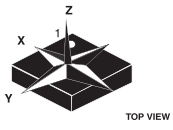
\includegraphics{fig/compass.png}%[width=1.0\textwidth]
	\label{fig:IMU_com}
	\caption{Compass, Source: Data sheet}
\end{figure}


\subsection{Gyroscope Sensor}

This sensor gives information about the angles of all axis, how the quadrocopter lays in the air.\\
We check the work of sensor with observing the live data, as before.

\begin{figure}[H]
	\centering
		\includegraphics{fig/Gyroscope.png}%[width=1.0\textwidth]
	\label{fig:IMU_Gyro}
	\caption{Gyroscope, Source: Data sheet}
\end{figure}


\begin{figure}[H]
	\centering
		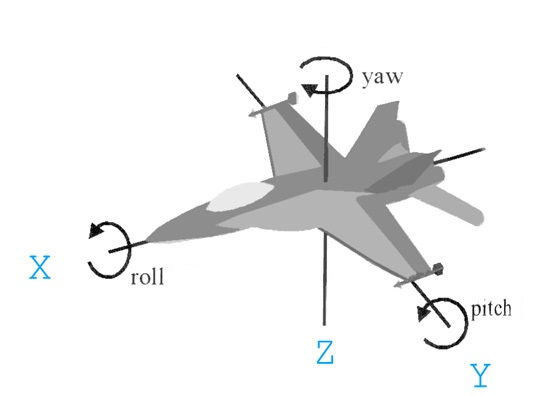
\includegraphics[width=0.7\textwidth]{fig/timzaman.jpg}%
	\label{fig:IMU_Gyro}
	\caption{Example at plane, Source: timzaman.com}
\end{figure}



\subsection{Pressure Sensor}

This sensor delivers a height compared to the sea level. You can say it is a absolute value.
For that reason it easy to place the sensor at certain heights, and took a lot of data. So we can see the jitter. When lifting it up/down fast for several meters, we can check how fast we get the updated data.

In future this sensor will be controlled with the data form the distance measurements to the ground under us. So we can eliminate the influences from the weather for example.



%\chapter{Realisierung}
%\label{sec:real}
%Beschreibung der HW- und SW-Realisierung
%
%\section{Unter-Kapitel in Realisierung}
%\label{sec:real-unter}
%Beispiel Text
%
%
%\newpage
%\section{Weiteres Unter-Kapitel in Realisierung}
%\label{sec:real-unterWeiter}
%
%\newpage
%\section{Und noch ein Unter-Kapitel in Realisierung}
%\label{sec:real-unterWeiterNoch}
%
%\section{Literaturverweise}
%\label{sec:real-literatur}
%
%Verweise im Text: \cite{doc:stz} und \cite{doc:gun}.
%
%\chapter{Ergebnisse}
%\label{sec:ergeb}
%\enquote{Neuigkeiten} Messergebnisse

% Bsp. eines Hauptteils

\chapter{Landing Concept}
\label{cha:LandingCon}


This Chapter is about the (theoretical) ways, how to manage a autonomous landing.

In anyway we need to adjust the speed of the rotors, depending on our measurements.


\section{Challenges}
\label{sec:landcha}

There will be several critical "challenges" during a landing process. Some of them when can estimate before and give a option, how to handle them.


\subsection{Drift}

It is very hard, to keep a Quadrocopter (in our case HElikopter) on a fixed point in a room. There is alway a little bit of wind, at least from the Quadrocopter itself. Therefore you always need to correct you position, to avoid it drifting away to one side.\\
With our sensors implemented we can recognize the movement and take some countermeasures.\\

The GPS system won't work indoor, so we need to rely on the IMU (Inertial Measurement Unit). So there is no absolute measurement of the position and we need to do some calculation with the acceleration in XY-Axis, to handle the drift.\\

With the gyroscope we can also handle the drift about our own axis.


\subsection{Orientation}

Because of our limited sensors, and a non working GPS indoor, it will not be possible to get a absolute orientation in a room.\\

Outdoors we can take the GPS with the barometer, the gyroscope and the laser sensor to get a very good knowing of where we are.


\subsection{Distance}

In a steady flight situation, we measure the distance straight to the ground. But when the quadrocopter is moving, we need to calculate the distance to ground with the angle of it.


\subsection{Landing Zone}

The first step will be, to take control of the landing watching with our eyes. Just decreasing the speed of the motors (rotors) depending on the distance to ground.\\

When we try that the Quadrocopter takes care of a free landing zone by itself, we can think about different options:\\

\underline{Circling}

With this method we just fly over the whole landing zone, which is a big as the quadrocopter. When we got the same distance value for the whole area, we can assume that there is no obstacle within it.


\underline{Remembering}

If we take some measurements during normal flight mode, we can save that values and try to build a map of the area under us. With this method we can fly to a "free" landing zone, when the landing mode is enabled.

\underline{lateral buckling}

May be the fastest and the most difficult way to land. By lateral buckling/tilting and calculation of the gathered values (depending on the angle), we can get a fast look over the area under us.

The challenge will be to stay, more or less, on the same position. Considering a certain height, where doing this action, there may be needed only small angles to tilt.

Or we could think about, mounting the laser sensor with a small angle. So to speak with a offset. We can easily consider the angle in the calculation of the height and only need to turn on the quadrocopters z-axis to check the landing zone.

\newpage
\section{Landing Mode}

The Landing mode should handle the landing of the quadrocopter fully autonomous.

\subsection{Activation}

The Landing Mode will/must be activated external. With it some sensor could be activated too, or configured in a other way. 


\subsection{Abort Landing}

We should be able to abort the autonomous landing, if we detect a problem.

1. approach: Just turning the Landing Mode off.

2. approach: Override the Landing Mode with the remote control.

3. approach: Abort the landing and turn the rotors off, to prevent damage to them.




%Verweise im Text: \cite{doc:stz} und \cite{doc:gun}.

\chapter{Open Points}
\label{sec:ergeb}

There are several points we wanted to do, but could not manage to do or finish them in time.

\section{Connecting sensors and actuators}

We did not connect any actuator, like an rotor, to our current software. There was no software ported to our Raspberry Pi to test with our developments.



\section{Reacting on sensor values}

There was no development to react in any way to our provided sensor values.


%\enquote{Neuigkeiten} Messergebnisse





% % %%%%%% Anhang
\appendix

%\chapter{Kapitel im Anhang}
\label{sec:a-kapitel}

Alles was den Hauptteil unn�tig vergr��ert h�tte, z. B. HW-/SW-Dokumentationen, Bedienungsanleitungen, Code-Listings, Diagramme


% % %%%%%% Literaturverzeichnis (darf im deutschen nicht in den Anhang!)
% Einfaches Literaturverzeichnis
%\begin{thebibliography}{XXXX}
%\bibitem{doc:stz} Thomas Nonnenmacher, LaTeX Grundlagen - Setzen einer wissenschaftlichen Arbeit Skript, 2008,\url{http://www.stz-softwaretechnik.de}; \textit{(Bei STZ Internetseite unter Publikationen - Skripte) [V.\,2.0 26.02.08]}
%
%\bibitem[Gun04]{doc:gun} Karsten G�nther, LaTeX2 --- Das umfassende Handbuch, Galileo Computing, 2004, \url{http://www.galileocomputing.de/katalog/buecher/titel/gp/titelID-768}; \textit{1. Auflage}
%\end{thebibliography}

% Literaturverzeichnis mit Bibtex
%\bibliography{bib/bib}

% %  Inhalt ENDE %%%%%%%%%%%%%%%%%%%%%%%%%%%%%%%%%%%%%%%%%%%%%%%%%%%%%%%%%%
\end{document}